\documentclass[conference]{IEEEtran}
\usepackage{times}
%\usepackage{durhampaper}
\usepackage{harvard}
\usepackage{graphicx}
\usepackage{tabu}

\citationmode{abbr}
\bibliographystyle{agsm}

\newcommand*\rot{\rotatebox{90}}
\def\tablename{Table}
\def\figurename{Figure}

\title{Time Frame Trading Algorithms}
\author{A. L. Gillies\\ M. R. Gadouleau\\ MEng Computer Science}

\iffalse
\title{Time Frame Trading Algorithms}
\author{A.L. Gillies}
\student{A.L. Gillies}
\supervisor{M. R. Gadouleau}
\degree{MEng Computer Science}
\fi

\date{}
\begin{document}
\maketitle

\thispagestyle{plain}
\pagestyle{plain}

\noindent
\begin{abstract}
\iffalse
The abstract must be a Structured Abstract with the headings {\bf Context/Background}, {\bf Aims}, {\bf Method}, {\bf Results}, and {\bf Conclusions}.  This section should not be longer than half of a page, and having no more than one or two sentences under each heading is advised.\\
\fi

Algorithmic trading is characterised by an entirely hands-off approach to stock market trading. All data manipulation, mathematical inference, machine learning and trade execution is done autonomously. With this approach, how much of an improvement can be gained over a standard interest rate provided by a high street bank, in the time frame given?

Using the average interest rate calculated from British banks in conjunction with implementation of both statistical and machine learning techniques shows that algorithmic trading can improve the annual return on investment over a given time frame.

This paper will consider two possibilities for implementation of the system: a purely statistical method, relying on known practices and techniques, and a hybrid system incorporating both statistical reasoning and machine learning. The known statistical practices are mostly used by human traders to allow for data insight and are well vetted. \cite{Murphy1999} The machine learning techniques are widely used in other contexts, with limited academic papers being available for this area.

The Support Vector Machine that made up the Machine Learning component of the testing outstripped all statistical methods by a significant margin, which in turn returned significantly higher results than are available through any high street bank.

This project was a success but contains an unbound task. There is always going to be a better method. The methods used within this paper are the result of limited time and resources: any extension to this project would reduce these limitations. Possible extensions include a wider range of machine learning techniques and using data of a finer grain, over a wider time frame.\\

\noindent
Keywords - Algorithmic, Machine Learning, Statistics, R, Trading, Stocks

\end{abstract}

\iffalse
#################################################################################
\fi

\section{Introduction}

\iffalse
This section briefly introduces the general project background, the research question you are addressing, and the project objectives.  It should be between 2 to 3 pages in length.  Do not change the font sizes or line spacing in order to put in more text.

- Same as the aims just longer.\\
- What is the aim for a year?\\
- Objectives.\\
- What is the state of the art in the field?\\
- A bit of the history of trading.\\
\fi

The stock market has been an early adopter of technology since its inception, as companies want to get an edge over their fellows and thus earn the most money. The first computer usage in the stock market was in the early 1970s with the New York Stock Exchange introducing  the Designated Order Turnaround system (DOT). This allowed for bypassing of brokers and routed an order for specific securities to a specialist on the trading floor \cite{Hasbrouck}. The definition of `broker' is an entity that buys and sells goods or assets for others, in this case `securities' which are defined as a financial instrument that holds monetary value. Since this point the use of machines to allow for increase throughput and speed has been pandemic. It was inevitable that computers would be used to aid the decision making process of what to buy or sell and when. This was shown to be very effective and recieved significant traction in the financial market in 2001 with the showcase of IBMs MGD and  Hewlett-Packard's ZIP \cite{Tesauro2001}. These two algorithmic strategies were shown to consistently outperform their human counterparts. They were both based on papers from 1996 showing that academic conception of algorithmic applications in financial markets has been present for several decades \cite{Gjerstad1998}, \cite{Cliff1998}. Whilst in the current day over one billion shares are traded every day, this would not be possible without computerised assistance. 

The aim of any algorithmic trading system is to `beat the market': is to buy low and sell high to gain the most capital over any given time frame, be that a day, a year, or a decade. This paper will look into the challenge faced by these algorithms and if, using available tools, it is possible to outstrip any high street banks offering rates. This will be achieved through simulation of a stock market, using real stock data, and the simulation of buying and selling these stocks using an algorithm. The current base bank interest rate is set at 0.5\% by the Bank of England \cite{BankofEngland2014}, with the average individual savings account or ISA over a fixed term of 1 year having a value of 1.85\% \cite{Murray2018}

\setlength\extrarowheight{2pt}

\begin{table*}
\centering
\begin{tabu}{ |l|l|p{10cm}| }\hline\hline
Unique ID & Deliverable & Description \\ \hline
DL1 & Simulate the financial market & Have data for at least 10 companies for at least a year, with data for each minute where data is available. \\ \hline
DL2 & Allow buying and selling of stocks & Have a functional buying and selling mechanism, with the data collected for each transaction processed. \\ \hline
DL3 & Implement statistical methods & Implement as many statistical methods as are beneficial to allow for the insight into the data for each stock. \\ \hline
DL4 & Implement a purely statistic strategy & Using just the statistical methods implemented in DL3, create a strategy that will buy and sell stocks to maximise profit made over the time frame given. \\ \hline
DL5 & Create a hybrid strategy & Implement a machine learning trading strategy that uses the stock data as well as any statistical methods that are helpful to maximise profit made over the time frame given. \\ \hline
DL6 & Implement tracking systems & Implement graphical and table outputs for the results of the computer logic and trading performance. \\ \hline
DL7 & Create a testing criteria & Create a method with which to test the strategy so as to avoid over fitting. \\ \hline
\end{tabu}
\vspace{2 mm}
\caption{Deliverables}
\label{fig: Tables Deliverables}
\end{table*}

This project will be based around the deliverables in table \ref{fig: Tables Deliverables}.

\iffalse
#################################################################################
\fi

\section{Related Work}

\iffalse
This section presents a survey of existing work on the problems that this project addresses.  it should be between 2 to 4 pages in length.  The rest of this section shows the formats of subsections as well as some general formatting information for tables, figures, references and equations.
\fi

\iffalse
The related work in this field is limited. This is due to the state of the art being controlled by large companies that use the work within this field to make money and being the state of the art means that the company that has it will make the most money, resulting in a limited flow of information on anything that is state of the art, as any sharing of information will result in that edge being lost and any money that was being made along with it. There are papers that exist that are seen as classic within the academic field of trading but within the world of algorithmic trading past papers are seen more as a has-been example of what was done in the past and bares little fruit with relevance to what is being done today. \\

Classic financial papers such as those that include the Black-Scholes Model \cite{Saad2015} are seen as pivotal in the study of academic finance and have been read by many within the financial world but offer very little in the way of help for computational finance. The same can be said for papers that cover the application and implications of Brownian motion, or the effect of the Efficient Market Hypothesis \cite{Meng2016}. Both very applicable to the modern world of finance as a whole, but almost unusable within the context of this paper. \\

Books published within the last decade are so far out of touch with the `Electronic and Algorithmic Trading Technology - The Complete Guide' \cite{Kim2007}, released in 2007 provides a very detailed description of all routing and pair trading techniques that are being used by a stock exchange to facilitate trading in the modern day and a long history of the adoption of algorithmic trading. But any strategies that are suggested are based on volume weighted average or time weighted average and have already been tested thoroughly. But are not ground breaking or competitive within modern markets. Other publications that have been found show similar limitations. Papers based around any machine learning techniques focus on k-means clustering \cite{Gerlein2016} or the Ising model \cite{Lima2017}, the Monte-Carlo or Wolff algorithm especially, have been thoroughly explored and show thorough testing in modern markets are not as competitive as they once were. Any paper that uses a different technique or shows the theoretical possibility of using many techniques in conjunction does not provide data or tangible results for any of the techniques instead suggests theoretical applications and limited or narrow real world applications.\\

Within this paper the statistical methods used have been found through papers that explore any data insight model that have been outlined within papers in the last half century, and are still useful within the modern day. These are basic `bread and butter' methods that are useful but not ground breaking. The machine learning technique has been shown to work as well as any other in theory and so will be tested more rigorously.\\
\fi

As has been mentioned previously, this field is made up of companies or researchers that are unwilling to share their recent breakthroughs. This results in a copious amount of research being available for techniques that are seen as antiquated, with very little being published on state-of-the-art. Any modern technique being employed is done so by an institution which uses it to profit from the stock market, this `edge'  will be guarded until it is no longer useful.

The available papers that are based in this field are focused on statistical implementation. With multiple books being published on the topic. Some based on single strategies but most being compendiums of multiple strategies, for example \cite{Murphy1999}. There are a few papers that include more complex models such as the Black-Scholes Model \cite{Saad2015} which are seen as pivotal to the world of economics and finance, but have little benefit to computational finance. The same can be said for papers concerning the application and implications of Brownian motion, or the effect of the Efficient Market Hypothesis \cite{Meng2016}. Although applicable to the modern world of finance as a whole, they are almost unusable within the context of this paper. This is due to the highly fluid and abstract nature of these theorems that are used to try to explain the world of economics more as a whole instead of giving finer details on more specific topics within this area.

This results in a juxtaposition of copious amounts of research into the statistical methods that are available and their reasoning, with a significant paradigm shift into the research that is based around machine learning in this context.

The most useful piece of research for the statistical methods is \cite{Murphy1999}. This book is a compendium of trading strategies that were used in the time period of 1950 to 1980, with ample detail on market analysis and any charts readable by humans that can be used within a trading scenario, whilst also giving details of the philosophy behind the trading. It also compares the use of computerised aids within a financial market to a purely human system. Electronic and Algorithmic Trading Technology \cite{Kim2007} contains multiple strategies and specific statistical methods that are useful within this context. It also shows a significant amount of detail concerning the surrounding systems, for example matching software that is used within a stock exchange that is not relevant. Written more from the view of a stock exchange, significant time and detail is given to the automation of`order flow' more commonly known as the matching of buying and selling parties within a stock exchange. Trading Commodities and Financial Futures \cite{Kleinman2005} is written very much for the purpose of teaching human traders. With sections on the psychology of trading and the history of trading. The techniques used can also be applied within computerised finance and are discussed in great depth. `Dark markets asset pricing and information transmission in over-the-counter markets' \cite{Duffie2012} contains very little in the way of strategies but is useful to give a wider picture of the context and legal aspects of trading. The data aspect touched upon within this book is very useful in inspiring the data formatting and data manipulation that is to be used throughout this paper.

The limiting factor for papers within this domain is that they are not within the field of machine learning in addition to being within the domain of computer finance. The inverse can be said for papers within the field of machine learning. Those that fall into both categories are limited in other ways. Some being too general to be of significant use, others being more in line with an academic look at the history of the domain. `Evaluating machine learning classification for financial trading: An empirical approach' \cite{Gerlein2016} is one of the papers that was found to have test results but was limited in that no strategies were provided and very little detail is given about the very basic models that are employed within the paper. The point is made that complex models have downsides and that Occam's Razor may play a role. `Predicting Stock Price Direction using Support Vector Machines' \cite{MadgeAdvisor} is a very relevant paper that provides insight into the predictive powers of an SVM when used in conjunction with momentum and volatility measures. \cite{MadgeAdvisor} is limited in that testing was done with very general data and shows very little promise with respect to short term predictions. `Visual knowledge discovery and machine learning for investment strategy' \cite{Wilinski2017} is very useful in providing detailed information regarding machine learning data manipulation before input but does not specify any details of machine learning, just that it will be used in future. `Buy Low, Sell High: A High Frequency Trading Perspective' \cite{Cartea2014} is based within the world of High Frequency trading and whilst this would be useful to an extension of this paper, we do not take into account market reactions to actions taken within this paper so it is beyond the scope of this paper.

\iffalse
#################################################################################
\fi

\section{Solution}

\iffalse
This section presents the solutions to the problems in detail.  The design and implementation details should all be placed in this section.  You may create a number of subsections, each focussing on one issue.
This section should be between 4 to 7 pages in length.
\fi

The solution is outlined in several sections that split the task into the stages that were followed in order to test the viability of all claims within this paper.

\iffalse
#################################################################################
\fi

\subsection{Simulation}

This section will outline in detail all components of the simulation and their interconnectivity. The purpose of this section is to give details on all work that was done outside of the implementation of the algorithms tested. Simply implementing the mathematics would not allow for testing of these algorithms. 

\subsubsection{Methodology}

The logic behind the simulation was to allow trading at a fine grain level, which needed to be permitted by the data used to perform the algorithms. The data that was available grows from `tick data' or data for every trade executed, to 'minute data`, giving details of all trades within that minute, and growing to 'day data` and beyond, which are all the same as minute but with a widening ranges. A drawback was that `tick data' was found to be too costly for the project so `minute data' was used. Minute data provides an open, high, low, and close price for a stock in the given minute, which gave plenty of data points per day of trading. A simplification was created at this point, trading was only done on the price that opened the minute. This was done to reduce the complexity of calculating any inter-minute values. The running of the simulation was based on the progression through each date of available trading and for each day iterate through every minute of the trading day, starting at 09:30 until 16:00. Each trading day has 390 points at which trading is possible, if the data permits it. This is available for 382 days in the 18 months of data that was used. 

The programming language that was chosen for this task was R \cite{Team2013}. This was chosen over other languages due to its extensive data manipulation capabilities as well as the contained mathematics functions such as standard deviation and differentiation. The data manipulation allows for large sets of incomplete data to be sub-sampled and manipulated into a usable form. The mathematical functions will form a basis for the statistical methods that are to be implemented.

\subsubsection{Data}

45 different stocks were used in this paper, taking from each the maximum number of data points available between 01/03/2016 and 01/09/2017. This gave an 18 month window wherein the first 6 months did not allow for trading to occur, only for data collection and training of models (which will be discussed in depth further in the paper) and the final 12 months were allocated for testing each algorithmic approach. There were some limitations with the data that was used. Due to the volatility of the stock market and the fact that some days trading was halted for a myriad of reasons, the target of 390 data points per day, for 18 months, was not achieved. Trading is not available on weekends, on bank or national holidays, or if trading is halted for some other reason. This meant that the solution had to take into account holes in the data. These gaps are also not regular: any given day can be cut short or a whole day could be taken without a pattern. Gaps also exist in minutes in  which no trades were executed. Which removes any values from the data and removes the possibility of trading within these minutes.

The data was taken from the NASDAQ, the second largest stock market in the world. The number of stocks used was arbitrarily big enough to provide enough data to test any given algorithm, some of which were found to prefer an abundance of data whilst others were much more short sighted and volatile. The most frequently traded stocks were chosen to allow for the most complete data.

The data was first downloaded in the form shown in Table \ref{fig: Table Data Input}, it was then converted using an R script into the form shown in Table \ref{fig: Table Data Formatted}. Thus reducing computational overhead from running the simulation as all data manipulation had been done prior to the data being used. In the final form no other alterations had to be made to the data other than set data types. 

Some examples of the formatted data in use can be seen in Figures  \ref{fig:AXP Stock Price},\ref{fig:IBM Stock Price},\ref{fig:MSFT Stock Price},\ref{fig:YAHOO Stock Price},\ref{fig:AA Stock Price},\ref{fig:AMAT Stock Price},\ref{fig:HD Stock Price}, and \ref{fig:MCD Stock Price}.

\begin{table*}
\centering
\begin{tabu}{ |p{1.5cm}|p{1.5cm}|p{1.5cm}|p{2cm}|p{2cm}|p{2cm}|p{2cm}| }\hline\hline
Ticker & Date & Time & Open & High & Low & Close \\ \hline
AA & 01/03/16 & 09:30 & 9.1100000 & 9.1300000 & 9.1100000 & 9.1100000 \\ \hline
AA & 01/03/16 & 09:31 & 9.1000000 & 9.1200000 & 9.0800000 & 9.0900000 \\ \hline
... & ... & ... & ... & ... & ... & ... \\ \hline
\end{tabu}
\vspace{2 mm}
\caption{Data of a single stock, in this case AA.}
\label{fig: Table Data Input}
\end{table*}

\begin{table*}
\centering
\begin{tabu}{ |p{1.5cm}|p{1.5cm}|p{2cm}|p{2cm}|p{2cm}|p{2cm}|p{1.5cm}| }\hline\hline
Date & Time & AA & AAPL & ADBE & AIG & ... \\ \hline
01/03/16 & 09:30 & 9.11 & 97.66 & 86.15 & 50.59 & ... \\ \hline
01/03/16 & 09:31 & 9.10 & 97.58 & 86.22 & 50.67 & ... \\ \hline
... & ... & ... & ... & ... & ... & ... \\ \hline
\end{tabu}
\vspace{2 mm}
\caption{Formatted data of all stocks used.}
\label{fig: Table Data Formatted}
\end{table*}

\begin{figure}
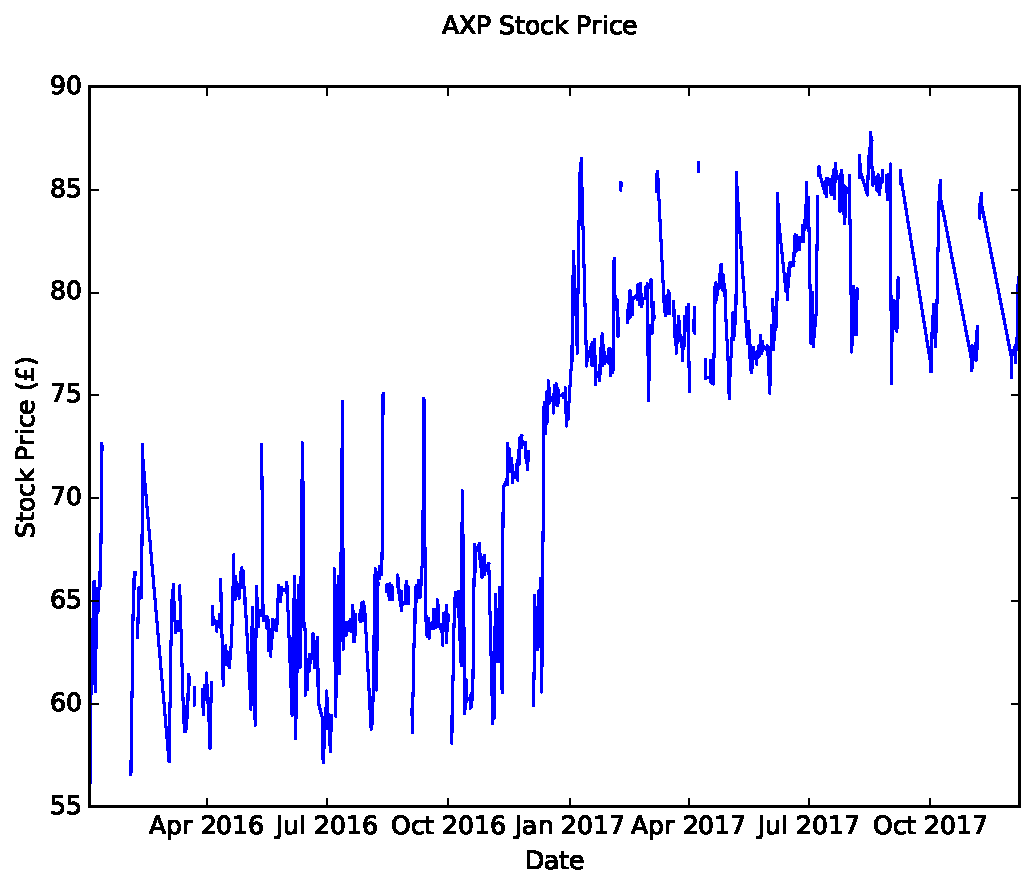
\includegraphics[width=0.5\textwidth, angle=0]{AXP.pdf}
\caption{A graph showing the AXP stock price over the time frame used.}
\label{fig:AXP Stock Price}
\end{figure}

\begin{figure}
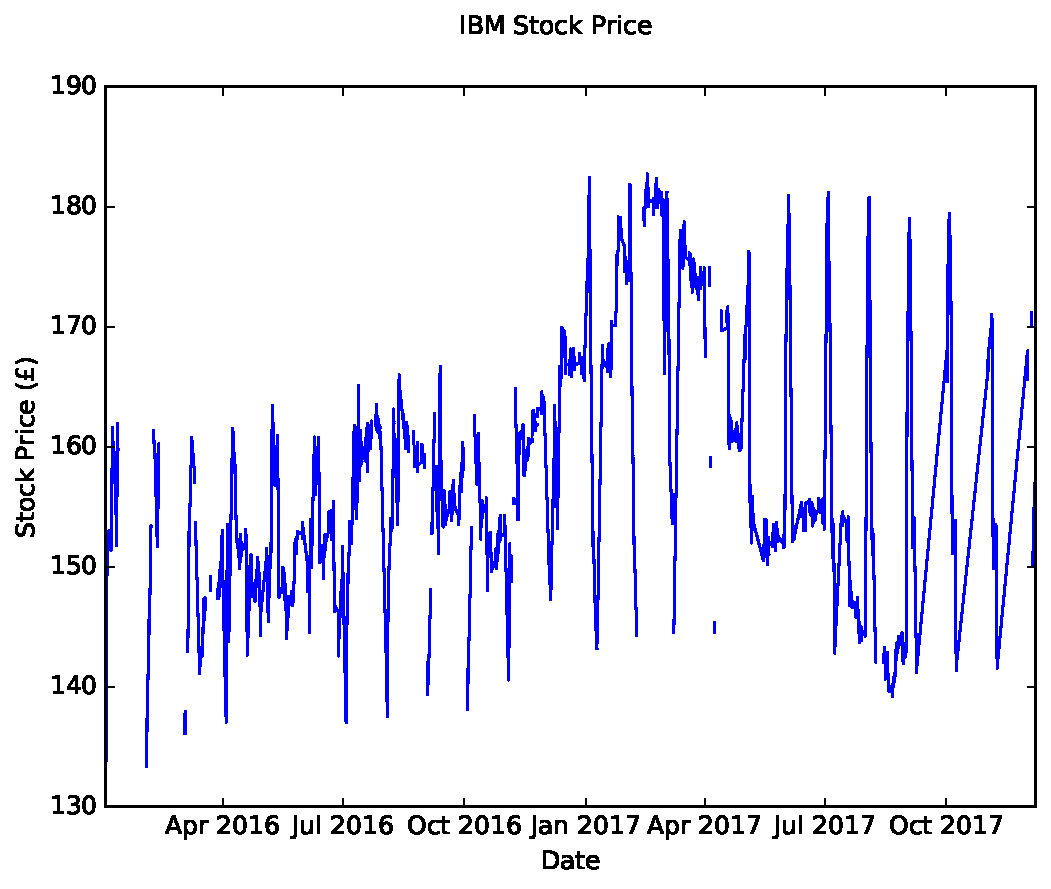
\includegraphics[width=0.5\textwidth, angle=0]{IBM.pdf}
\caption{A graph showing the IBM stock price over the time frame used.}
\label{fig:IBM Stock Price}
\end{figure}

\begin{figure}
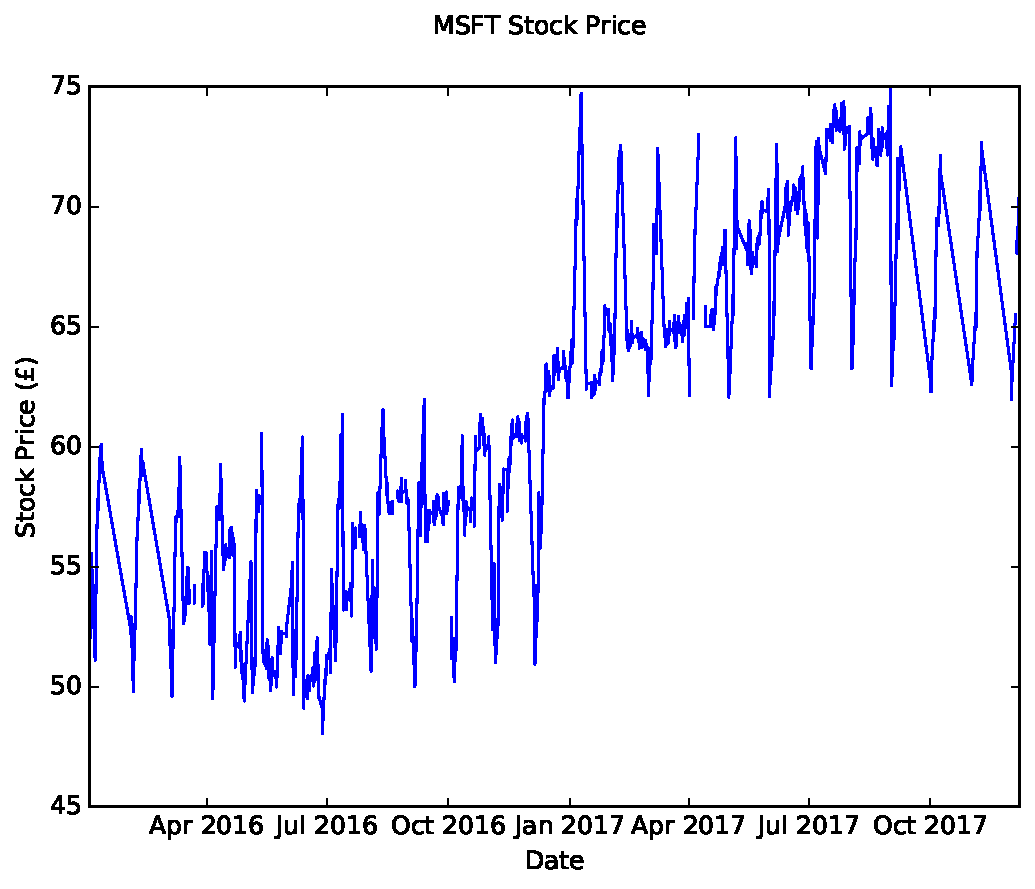
\includegraphics[width=0.5\textwidth, angle=0]{MSFT.pdf}
\caption{A graph showing the MSFT stock price over the time frame used.}
\label{fig:MSFT Stock Price}
\end{figure}

\begin{figure}
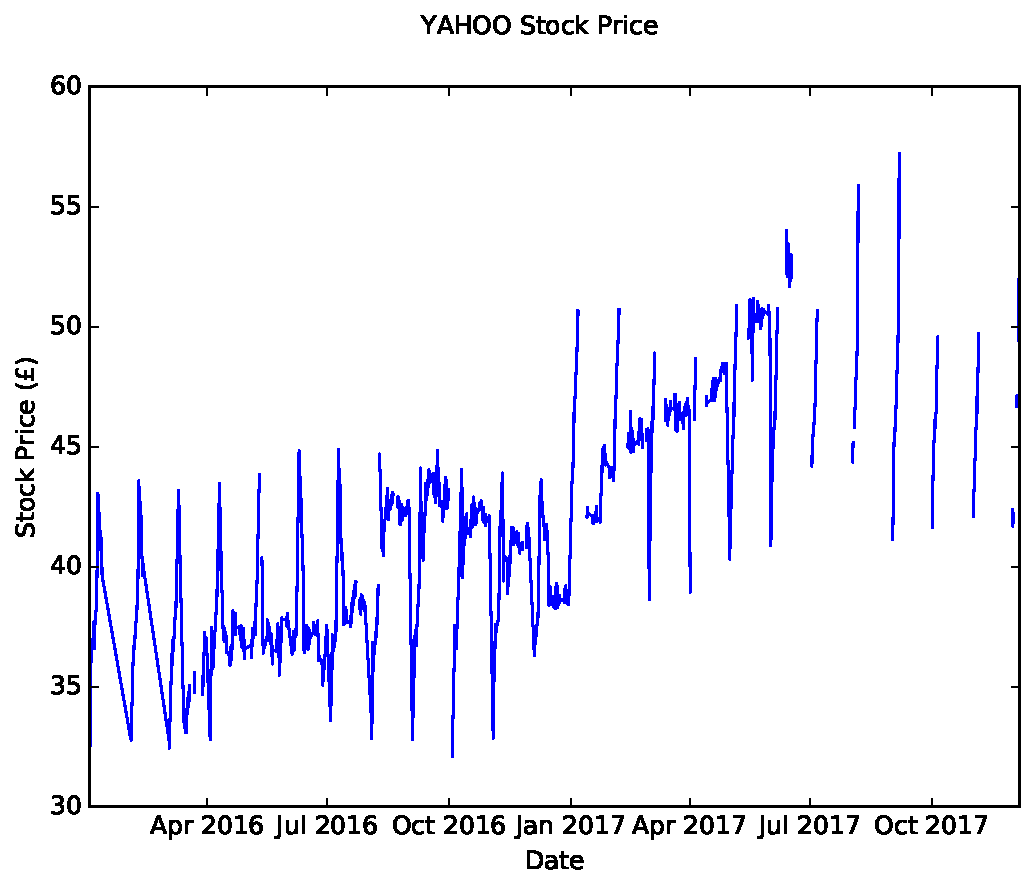
\includegraphics[width=0.5\textwidth, angle=0]{YAHOO.pdf}
\caption{A graph showing the YAHOO stock price over the time frame used.}
\label{fig:YAHOO Stock Price}
\end{figure}

\iffalse
################
\fi

\begin{figure}
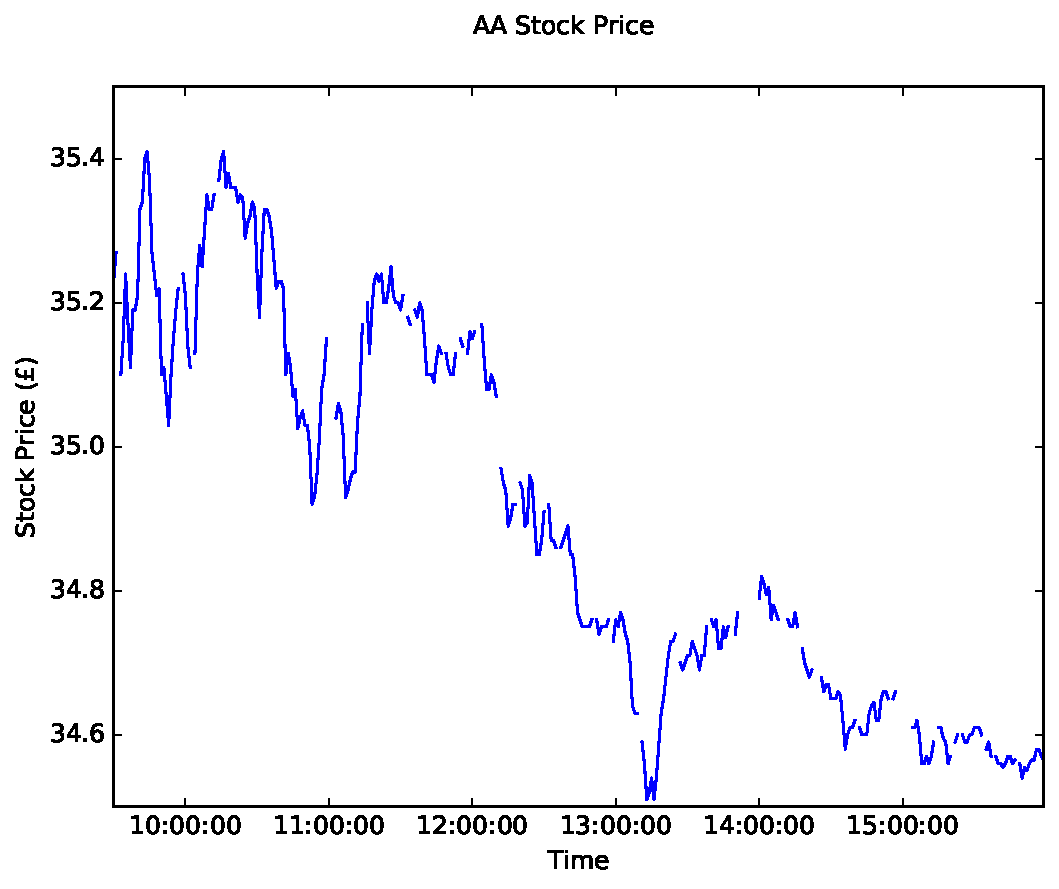
\includegraphics[width=0.5\textwidth, angle=0]{AA.pdf}
\caption{A graph showing the AA stock price over a single day.}
\label{fig:AA Stock Price}
\end{figure}

\begin{figure}
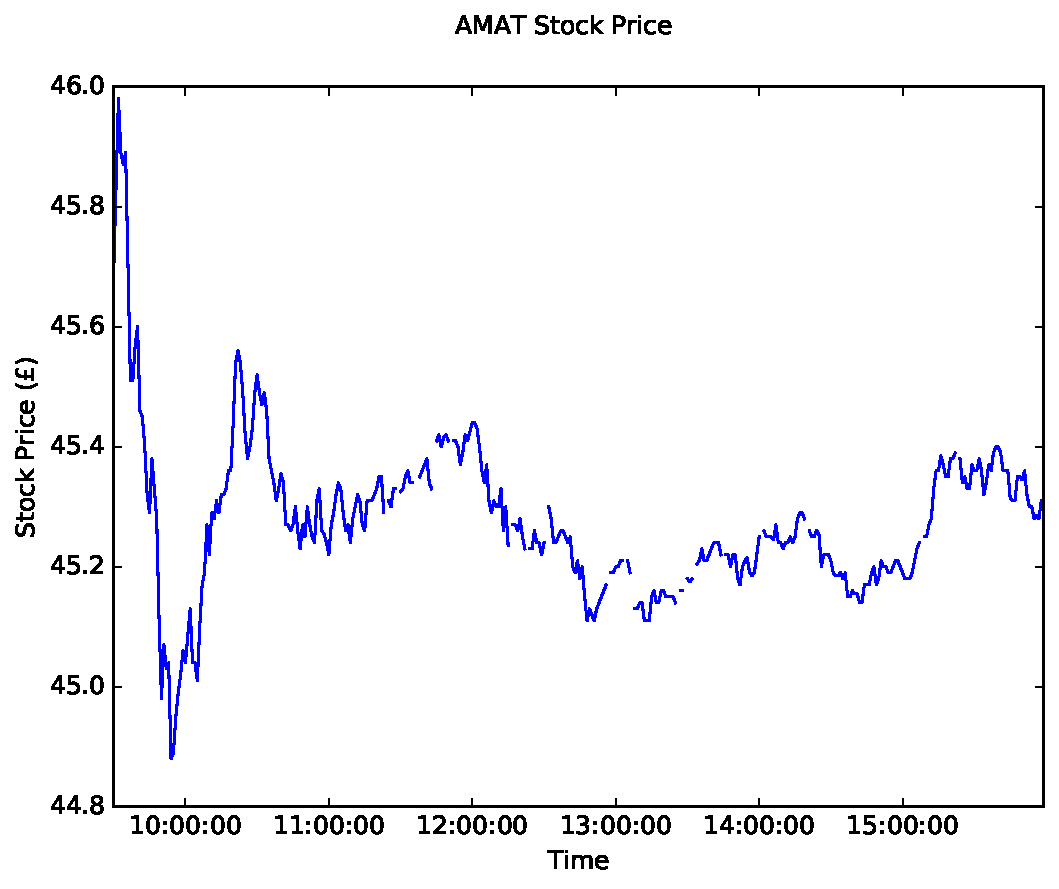
\includegraphics[width=0.5\textwidth, angle=0]{AMAT.pdf}
\caption{A graph showing the AMAT stock price over a single day.}
\label{fig:AMAT Stock Price}
\end{figure}

\begin{figure}
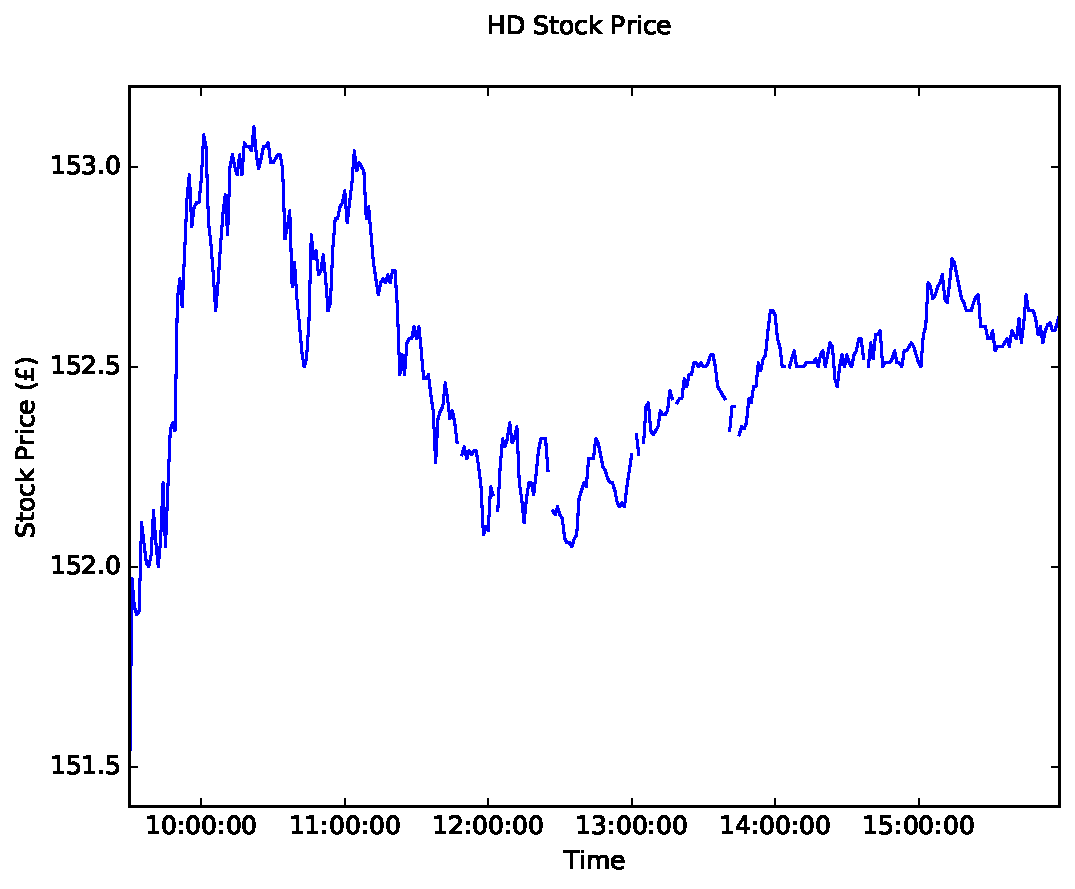
\includegraphics[width=0.5\textwidth, angle=0]{HD.pdf}
\caption{A graph showing the HD stock price over a single day.}
\label{fig:HD Stock Price}
\end{figure}

\begin{figure}
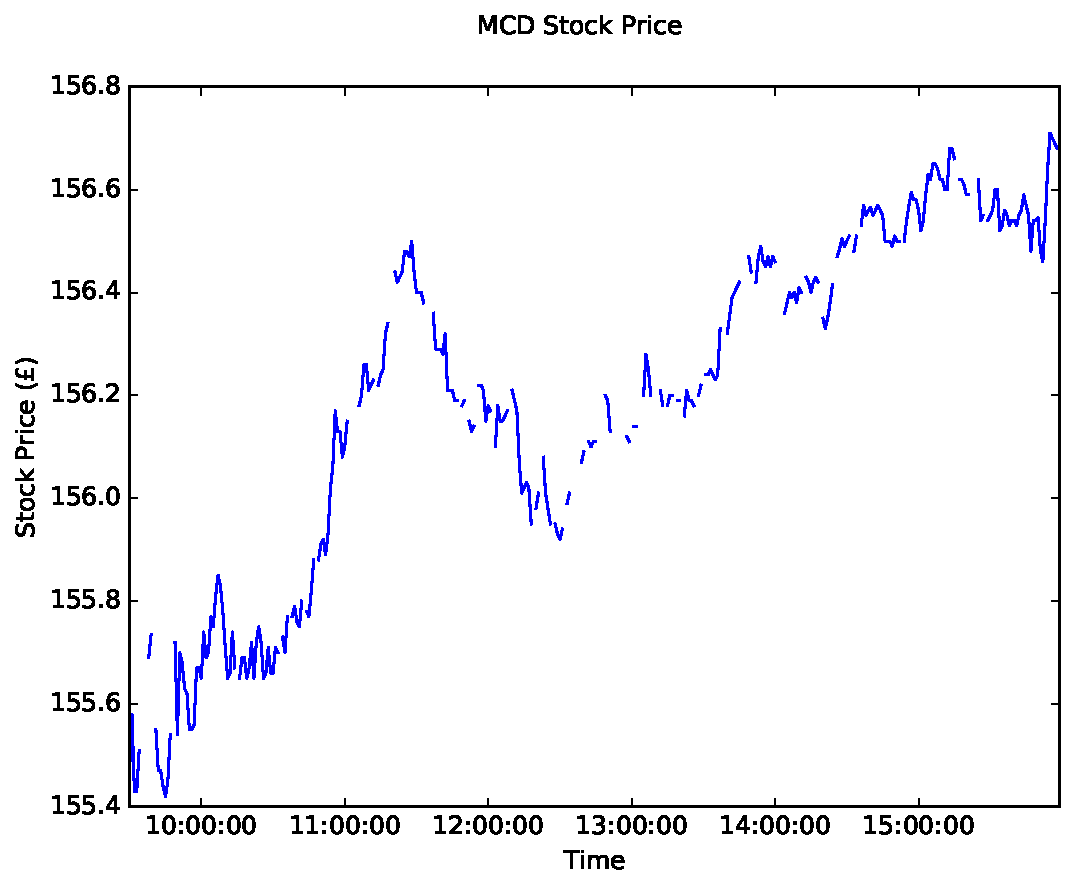
\includegraphics[width=0.5\textwidth, angle=0]{MCD.pdf}
\caption{A graph showing the MCD stock price over a single day.}
\label{fig:MCD Stock Price}
\end{figure}

\subsubsection{Set-up}

The simulation was set up in such a way so as to minimise the impact caused by gaps in the data. This meant using the data to provide the iteration behaviour. The data input in the form of Table \ref{fig: Table Data Formatted} was cast for each row using a typecast function to allow for correct manipulation of numerical values. The dates were converted to numerical values for correct comparison, as were the times. The stock values were also numerical. 

The simulation then uses all unique dates within the Dates column to allow for iteration through the table at the highest level, through each individual day. Once the data had been sub-sampled for that day, then a list of unique minutes was created. Once the data had been further sub-sampled to the current minute, each of the stock columns were iterated through and tested for NA, or Not Available, values. If an NA value is present for that stock, then it is passed over. If the value is available however then two functions are used, `shouldBuy' and `shouldSell'. The first used is `shouldBuy'; this will take input of current date, current time, and current stock, to allow for a decision to be made on whether to buy an amount of that stock or not. These functions are based on manipulations of three other tables, `Active', `Sold', and `Ledger'. These are shown in tables IV, V, and VI, respectively.

\begin{table*}
\centering
\begin{tabu}{ |p{2.25cm}|p{2.25cm}|p{2.25cm}|p{2.25cm}|p{2.25cm}|p{2.25cm}| }\hline\hline
Unique ID & Date Bought & Time Bought & Stock & Number of Shares & Cost per Share \\ \hline
... & ... & ... & ... & ... & ... \\ \hline
\end{tabu}
\vspace{2 mm}
\caption{Active}
\label{fig: Active}
\end{table*}

\begin{table*}
\centering
\begin{tabu}{ |l|l|l|l|l|l|l|l|l|l|l|l| }\hline\hline
\rot{Unique ID} & \rot{Date Bought} & \rot{Time Bought} & \rot{Stock} & \rot{No. of Shares} & \rot{Cost per Share} & \rot{Amount Bought} & \rot{Date Sold} & \rot{Time Sold} & \rot{Price per Share} & \rot{Amount Sold}\\ \hline
... & ... & ... & ... & ... & ... & ... & ... & ... & ... & ... \\ \hline
\end{tabu}
\vspace{2 mm}
\caption{Sold}
\label{fig: Sold}
\end{table*}

\begin{table*}
\centering
\begin{tabu}{ |p{2.25cm}|p{2.25cm}|p{2.25cm}|p{2.25cm}| }\hline\hline
Date & Total Value & Stock Value & Capital Value \\ \hline
... & ... & ... & ...  \\ \hline
\end{tabu}
\vspace{2 mm}
\caption{Ledger}
\label{fig: Ledger}
\end{table*}

Each also comes with its own population function, `Buy', `Sell', `Update'. The first two are called if any decision is made. If a stock's value is such that the `shouldBuy' function returns true then the `Buy' function is called, taking input of date, time, stock, and amount. The amount is dictated by the `amountShouldBuy' function that is an extension of the `shouldBuy' function that returns the amount of the current stock that should be bought. This is then added as another row to the `Active' table, as this is now an active stock that can be sold. The amount of any given stock that should be purchased is calculated through another function `getAmount'. This will test all calculations done in `shouldBuy' and calculate a confidence value that will then, using the amount of liquid capital available, dictate the amount of the stock that will be bought. The `shouldSell' function is then queried every time an updated value is available for any given row in the `Active' table. Using the new value a decision will be made if the stock should be sold, if this is found to be the case then the `Sell' function is called. The function will remove the row of the `Active' table that corresponds to this block of stock to be sold and add it to the `Sold' table along with all the details of the transaction. 

The final table is `Ledger' which uses the function `Update'. This is called on a regular basis to allow for tracking of the algorithm throughout the simulation. All overall details of capital are stored in this table. The `Date' column is a concatenation of both `Time' and `Date' in any other table to allow for minute by minute updates of the simulation or if this is not required then daily updates are possible.\\

\iffalse
The simulation was set up in an iterative way in order to minimise the disruptions that missing data would cause, whilst also being exhaustive and searching for data given a reference point is straightforward, so no data point is missed or an inaccurate search is done. A simple testing framework was set up during implementation, variable controlled which stocks were being iterated through at any given moment,what dates were available, when any trade execution could commence, and the amount of capital that was available to any given algorithm. Once these had been established then each date from the start date to the end date variables was found through merged table of all dates across all stocks as some stocks are available to trade when others are not, these are then iterated through. Within this loop is another very similar loop that performs the same action but for minutes rather than dates. All available times are found for the specific date, and iterated through. Finally, for each stock that is available, during testing not all stocks were used so as to help with the removal of bugs, instead a random number generator would choose a predefined number of stocks and iterate over these instead. A stock value is found for that date, at that time, for that stock. Once this has been done then then calculations can be made to decide if any action needs to be taken given this new information. Any buy or sell actions are handled by a single function each that will take in all current information, including the time, date, and stock price. These two functions shall be known as the `shouldBuy' and `shouldSell' functions throughout this paper. These functions will be given all available information and will then make a decision using the methods they have been assigned. Any action that is taken will be stored in tables set up before the simulation was started. There are three tables, initially only two were used but a third was introduced at a later date to increase the speed of execution of the simulation. These tables are `Active', `Sold', and `Ledger'. Active is any bundle of stocks that have been bought by the algorithm, stored as a row containing; A unique identifying number to allow for easy retrieval of the row, the date on which the stock was bought, the time at which the stock was bought, the name of the stock, the number of shares that were bought during this execution, and the cost per share or stock price as these are the same. This table is iterated through every time a new stock price becomes available for a stock that is present in the table and the `shouldSell' function is called, then any necessary calculations are done to decide if this bundle of stocks should be sold or not. If it is decided that this bundle should be sold then this row is removed from the `Active' table and added to the `Sold' table. This table contains the same headers as the `Active' table with the addition of the total amount bought, meaning number of shares multiplied by price they were bought at, the date sold on, the time sold at, the price per share that they were sold at, and the total amount sold. The two totals, total bought and total sold, may seem to be superfluous by they are relied upon by the final table. This table is the most used, it has a row added each time a change is made within the simulation regardless of any actions taken. Each minute a new row is added to this table to keep track of all capital that is within the simulation, the reason for this table is to show at the end of the simulation all trades that were performed and the amount of capital that is liquid or in stocks at any given moment. During implementation minute by minute updates were not required and this only served to increase the execution time of the simulation by a significant amount, and thus the function that adds a new row to this table was only called at the end of each day iteration instead of at the end of each minute iteration. This table contains the heading; date - this was a concatenation of both time and date with a simplified name, value - this was the total value within the simulation, stock value - this is the total amount of capital that are currently within stocks, and capital value - this is the amount of liquid capital available. \\

ADD THREE TABLES TO SHOW HOW THEY LOOK\\
\fi

\subsubsection{Functions}

Shown in Table \ref{fig: Table Basic Functions} are some of the more regularly utilised functions in the simulation and are the key underpinnings of the statistical and machine learning techniques that are used throughout the simulation. \\

\begin{table*}
\centering
\begin{tabu}{ |p{4cm}|p{4cm}|p{6cm}| }\hline\hline
Function & Arguments & Details \\ \hline
Buy() & Date, Time, Stock, Amount & Adds a row to the `Active' table.  \\ \hline
Sell() & Row Data, Date, Time, Stock, Stock Price & Adds a row to the `Sold' table and removes the corresponding row of the `Active' table.  \\ \hline
Update() & Date, Total Capital & Adds a row to the `Ledger' table for re-tracking of the simulation  \\ \hline
shouldBuy() & Date, Time, Stock & Calculates using any method set if the current stock should be bought at the current price.  \\ \hline
shouldSell() & Unique ID, Date, Time & Calculates if the given block of stocks should be sold at the current price.  \\ \hline
amountShouldBuy() & Date, Time, Stock & This is a function that is used to find a confidence value in the current stock price and thus returns the amount of the given stock that should be bought also taking into account the amount of liquid capital that is available at the current time.  \\ \hline
getMax() & List & Get the maximum value of the given list.  \\ \hline
getMin() & List & Get the minimum value of the given list.  \\ \hline
getAverage() & List & Get the mean value of the given list. \\ \hline
getSD() & List & Get the standard deviation of the given list.  \\ \hline
getXDate() & Date, X & Get the date X days ago  \\ \hline
getXClose() & Date, Stock, X & Get the close X days ago.  \\ \hline
getXOpen() & Date, Stock, X & Get the open X days ago.  \\ \hline
getXDataPoints() & Date, Time, Stock, X & Get the last X data points for the given stock  \\ \hline
getXDayDataPoints() & Date, Stock, X & Get all data for the day X days ago. \\ \hline
getXSincePrice() & Date, Time, Stock, Price & Get the number of data points between the current data point and the last data point that had the given price.  \\ \hline
getTotalGainLoss() & Date, Time, Stock, X &  Over the last X data points get the total gain and loss. \\ \hline
\end{tabu}
\vspace{2 mm}
\caption{Basic Functions}
\label{fig: Table Basic Functions}
\end{table*}

\iffalse
\noindent
\textbf{Buy}(Date, Time, Stock, Amount) - Adds a row to the `Active' table. \\
\noindent
\textbf{Sell}(RowData, Date, Time, Stock, StockPrice) - Adds a row to the `Sold' table and removes the corresponding row of the `Active' table.\\
\noindent
\textbf{Update}(Date, TotalCapital) - Adds a row to the `Ledger' table for re-tracking of the simulation.\\
\noindent
\textbf{shouldBuy}(Time, Date, Stock) - Calculates using any method set if the current stock should be bought at the current price.\\
\noindent
\textbf{shouldSell}(UniqueID, Date, Time) - Calculates if the given block of stocks should be sold at the current price.\\
\noindent
\textbf{amountShouldBuy}(Time, Date, Stock) - This is a function that is used to find a confidence value in the current stock price and thus returns the amount of the given stock that should be bought also taking into account the amount of liquid capital that is available at the current time.\\
\noindent
\textbf{getMax}(List) - Get the maximum value of the given list.\\
\noindent
\textbf{getMin}(List) - Get the minimum value of the given list.\\
\noindent
\textbf{getAverage}(List) - Get the mean value of the given list.\\
\noindent
\textbf{getSD}(List) - Get the standard deviation of the given list.\\
\noindent
\textbf{getXDate}(Date, X) - Get the date X days ago.\\
\noindent
\textbf{getXClose}(Date, Stock, X) - Get the close X days ago.\\
\noindent
\textbf{getXOpen}(Date, Stock, X) - Get the open X days ago.\\
\noindent
\textbf{getXDataPoints}(Date, Time, Stock, X) - Get the last X data points for the given stock.\\
\noindent
\textbf{getXDayDataPoints}(Date, Stock, X) - Get all data for the day X days ago.\\
\noindent
\textbf{getXSincePrice}(Date, Time, Stock, Price) - Get the number of data points between the current data point and the last data point that had the given price.\\
\noindent
\textbf{getTotalGainLoss}(Date, Time, Stock, X) - Over the last X data points get the total gain and loss.\\
\fi

\iffalse
#################################################################################
\fi

\subsection{Statistical Methods}

Once a working simulation had been established and all functions had been shown to be working, statistical methods had to be implemented. These were separated into two groups. The first are technical overlays, methods that provided insight into the data by providing numbers that are on the same scale as the price itself. Whilst the other group, technical indicators, give insight into the data through numbers that are in no way related to the stock price, and thus allow much more insightful comparisons to be made inter-stock as opposed to intra-stock. That is comparing two stocks is easier if technical indicators are used as opposed to using technical overlays which are very dependant on the stock price and do not translate as well to comparisons between two unique stocks. 

An example of a technical overlay is the Bollinger Band, the calculation of which will be shown in the following section. This technical overlay, shown in figure \ref{fig:HDDayBollinger}, clearly has an output range that is dictated by the stock price. An example of a technical indicator is the MACD, this will be explained further in the paper. This can be seen in figure \ref{fig:HDDayMACD} and shows that the stock price has no bearing on the final value of the indicator.

\begin{figure}
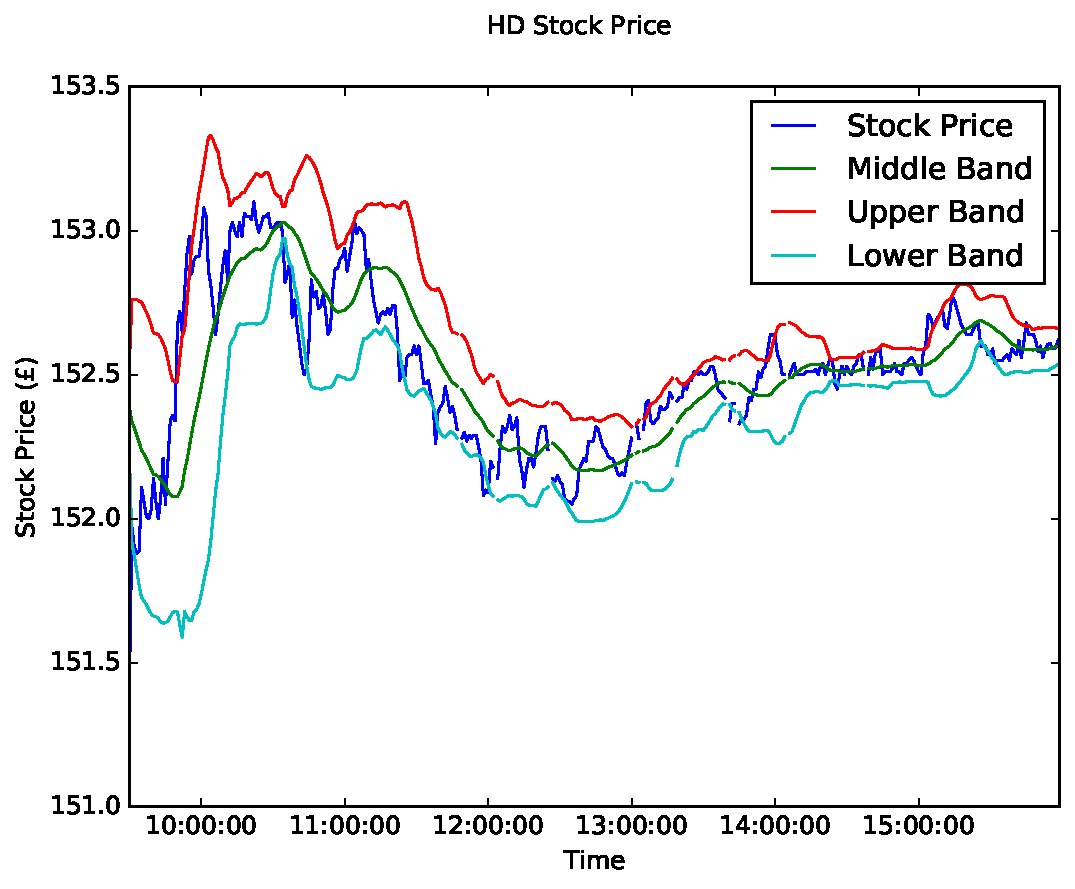
\includegraphics[width=0.5\textwidth, angle=0]{HDDayBollinger.pdf}
\caption{A graph showing the change in the value of Bollinger Bands as the value of the HD stock changes.}
\label{fig:HDDayBollinger}
\end{figure}

\begin{figure}
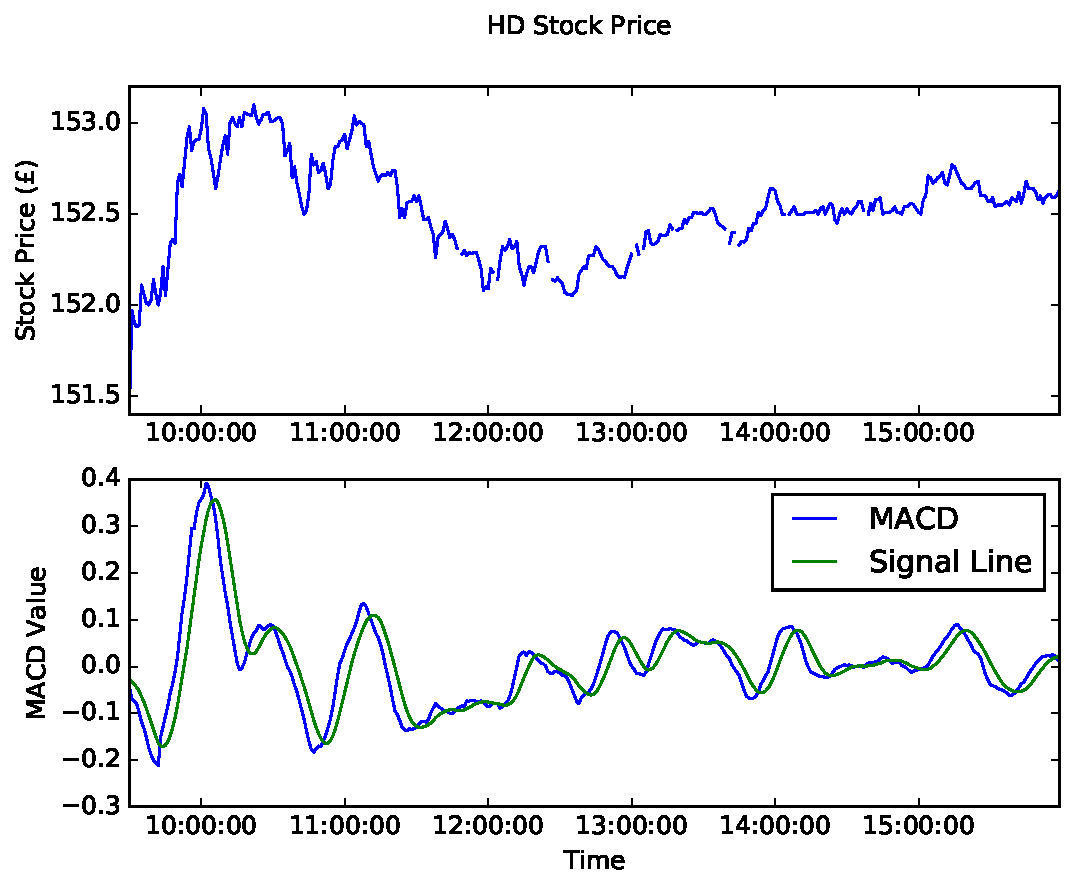
\includegraphics[width=0.5\textwidth, angle=0]{HDDayMACD.pdf}
\caption{A graph showing the change in the value of MACD as the value of the HD stock changes.}
\label{fig:HDDayMACD}
\end{figure}

\iffalse
#################################################################################
\fi

\subsubsection{Technical Overlays} Defined as a statistical method that is dependant on the price. \\

\textbf{Bollinger Bands} - \cite{Bollinger1992} - These are volatility bands placed above and below the current stock price and are based on the standard deviation. These are designed to give an indication of how the volatility of a given stock changes over time. For any given stock over a time frame X, the three bands are calculated as such:\\

\noindent
Upper band $=$ Simple Moving Average$(X)$ $+$ (Standard Deviation$(X) * 2$)\\
Middle band $=$ Simple Moving Average$(X)$\\
Lower band $=$ Simple Moving Average$(X)$ $-$ (Standard Deviation$(X) * 2$)\\
The standard time period is 20 days.

The complexity of these calculations is fairly low, with the upper and lower band being equidistant from the middle band. The middle band is a simple moving average from the last 20 days. This meaning that all values for the last 20 days are used to find the mean which is the value of the middle band. Standard deviation is a measure of how much a group of data differs from the mean of this data, in this case the values of the last 20 days. These are then used within the equations stated.\\

\iffalse
[]
\fi

\noindent
\textbf{Chandelier Exit} - \cite{Elder2002} - Developed by Charles Le Beau, this is designed to help stay within a trend and not to exit early. In the case of an uptrend the Chandelier Exit will typically be below the stock price and the inverse is true in the case of a downtrend. To calculate it over a time period X:\\

\noindent
Long = High(X) - (Average True Range(X) * 3)\\
Short = Low(X) + (Average True Range(X) * 3)\\
\noindent
The standard time period is 22 days.\\

The calculation of `High(X)' is done by taking the last X days of data and finding the maximum value. The `Low(X)' is calculated by finding the minimum value of the last X days of data. The average true range is shown in significant detail later in the technical indicators section.

\iffalse
[]
\fi

\noindent
\textbf{Ichimoku Cloud} - \cite{Murphy1999} - A multifaceted indicator developed by Goichi Hosoda, a Japanese journalist. This is an average based trend identifying indicator based on the standard candlestick charts. A candle stick chart is a method of showing the data for a given period in a graphical format using 4 data values. These are Open, Close, High, and Low. This indicator is used as a basis in a number of other theories including Target Price Theory. There are five plots within Ichimoku Cloud.\\

\noindent
Using time period X.\\
Tenkan-sen or Conversion line = (High(X) + Low(X)) / 2  - Default X is 9 days\\
Kijun-sen or Base line = (High(X) + Low(X)) / 2 - Default X is 26 days\\
Senkou Span A or Leading span A = (Conversion Line + Base Line) / 2 days \\
Senkou Span B or Leading span B = (High(X) + Low(X)) / 2 - Default X is 52 days\\
Chikou Span or Lagging span = CloseXPeriodsAgo(X) - Default X is 26 days\\

This is a much more complex calculation. `High(X)' and `Low(X)' are straight forward, but their use later in the calculation is more complex. The meaning of `CloseXPeriodsAgo(X)' is to find the final value of the day, X days ago. For example if X is 1, then the final value of the previous day is taken.\\

\iffalse
[]
\fi

\noindent
\textbf{Kaufman's Adaptive Moving Average (KAMA)} - \cite{Kaufman1998} - This indicator is designed to remove market noise during volatile periods. It takes three parameters, X, Y, and Z. X is the number of periods that is used by the first step of the calculation, known as the efficiency ratio. This will be shown later. The second is the number of periods for the first and fastest exponential moving average or EMA. Third is the number of periods for the second and slowest EMA. The defaults for these values are (10, 2, 30). \\

\noindent
Efficiency Ratio = Change/Volatility\\
Change = Absolute Value(Close() - CloseXPeriodsAgo(X)) - Default X is 10 \\
Volatility = Sum(Absolute Value(Close() - CloseXPeridsAgo(X))) - Default X is 1, this sum is done 10 times, for the last 10 changes in price.\\

\noindent
The next stage of KAMA is the calculation of a smoothing constant. 

\noindent
Smoothing Constant (SC) = ((Efficiency Ratio * (fastest SC - slowest SC)) + slowest SC)$^2$\\
The fastest smoothing constant is the calculation of an exponential moving average for the shortest period of time. The slowest smoothing constant is the EMA of the longest period of time. Typical value are 2 days and 30 days respectively.

\noindent
Final stage is the use of the previous KAMA value to calculate the next value. \\
New KAMA = Previous KAMA + (Smoothing Constant * (Current Price - Previous KAMA))\\

\iffalse
[]
\fi

\noindent
\textbf{Keltner Channels} - \cite{Keltner1960} - Very similar to Bollinger Bands but instead of using standard deviation average true range is used. Created by Chester Keltner, this indicator is made up of three lines in a similar way to Bollinger Bands.\\

\noindent
Upper Channel Line = Exponential Moving Average(X) + (2 * Average True Range(Y))\\
Middle Line = Exponential Moving Average(X)\\
Lower Channel Line = Exponential Moving Average(X) - (2 * Average True Range(Y))\\ Default X = 20, Y = 10 \\

The exponential moving average function finds the weighted average of the last X days. The weight is dictated by an exponential function with the final values having the most weight.\\

\iffalse
[]
\fi

\noindent
\textbf{Moving Averages} - \cite{Murphy1999} - These can come in multiple forms with multiple names. The catch-all term for this type of smoothing average is a moving average. The most simple is known as a Simple Moving Average (SMA). This takes the average of the last X data points. There is no weighting or extra steps. A more complex version is the Exponential Moving Average (EMA), this uses weighting to give the more recent values more significance in the calculation. The initial value of EMA is the same as the SMA for the same period as EMA requires an initial value.\\

\noindent
EMA$_{Today}$ = (Current Stock Price * K) + (EMA$_{Yesterday}$ * (1 - K)) \\
K = 2 / (N + 1) \\
N = Number of periods over which the EMA is applied \\

\iffalse
[]
\fi

\noindent
\textbf{Moving Average Envelopes} - \cite{Murphy1999} - Based on a Moving Average, this is a percentage based envelope that provides parallel bands above and below the Moving Average. Gives an indication of trends in the data as well as an indicator for stocks that are overbought and oversold when the trend is flat.\\

\noindent
Upper Envelope = MovingAverage(X) + (MovingAverage(X) * Y)\\
Lower Envelope = MovingAverage(X) - (MovingAverage(X) * Y)\\
Typical values X = 20 and Y = 0.025\\

\iffalse
[]
\fi

\noindent
\textbf{Parabolic SAR} - \cite{Wilder1978} - SAR stands for `stop and reverse', this was called a Parabolic Time/Price System. This indicator follows the stock price as the trend is formed, and will then `stop and reverse' when the trend ends, to follow the new trend. This is one of the more complex indicators.\\

\noindent
In the case of a rising SAR:

\noindent
EP or extreme point is a variable that is equal to the highest value of the current uptrend.\\
AF or acceleration factor is a variable that starts at 0.02 and is increment by 0.02 each time the EP is changed, meaning that it is incremented each time a new high is reached. The maximum value of AF is 0.2. \\

\noindent
SAR = SAR$_{Yesterday}$ + AF$_{Yesterday}$(EP$_{Yesterday}$ - SAR$_{Yesterday}$) \\

\noindent
In the case of a falling SAR:

\noindent
This uses the same variable names but inverse behaviour, the EP is equal to the lowest point in the current downtrend. AF is the same but is incremented when EP reaches a new low. \\

\noindent
SAR = SAR$_{Yesterday}$ - AF$_{Yesterday}$(EP$_{Yesterday}$ - SAR$_{Yesterday}$) \\

\noindent
These are used to indicate a trend and once a price falls to the other side of the value calculated in the current trend, that trend is over and SAR will flip to the opposite trend. \\

\iffalse
[]
\fi

\noindent
\textbf{Pivot Points} - \cite{Murphy1999} - An overlay used to indicate directional movement and then shows these in potential support and resistance levels. These are predictive indicators and they exist in multiple forms. The most well known are the standard, Denmark, and Fibonacci versions. These are calculated using the previous day's high, low, and close values and are then not recalculated throughout the trading day. A calculation has multiple components: the pivot point, multiple supports, and multiple resistances.\\

\noindent
Standard Pivot Points. \\
Pivot Point = (High + Low + Close)/3\\
Support One = (PP * 2) - High\\
Support Two = PP - (High - Low)\\
Resistance One = (PP * 2) - Low\\
Resistance Two = PP + (High - Low)\\

\noindent
Denmark Pivot Points. These are the most complex calculations as they have conditional statements in them and do not use the same calculation methods as the other two.\\
Pivot Point = X / 4\\
Support One = (X / 2) - High\\
Resistance One = (X / 2) - Low\\

\noindent
Where X is calculated as: \\
If Close $<$ Open: X = High + (2 * Low) + Close\\
If Close $>$ Open: X = (2 * High) + Low + Close\\
If Close = Open: X = High + Low + (2 * Close)\\

\noindent
Fibonacci Pivot Points. These are similar to the standard pivot points but use different spacing techniques, namely the Fibonacci sequence.\\
Pivot Point = (High + Low + Close)/3\\
Support One = PP - (0.382 * (High  -  Low))\\
Support Two = PP - (0.618 * (High  -  Low))\\
Support Three = PP - (1 * (High  -  Low))\\
Resistance One = PP + (0.382 * (High  -  Low))\\
Resistance Two = PP + (0.618 * (High  -  Low))\\
Resistance Three = PP + (1 * (High  -  Low))\\

\iffalse
[]
\fi

\noindent
\textbf{Price Channels} - \cite{Murphy1999} - Using three calculations to show an upper, lower, and middle bounds. Used to indicate the start of an upwards or downward trend.\\

\noindent
Upper = High(X)\\
Center = (High(X) + Low(X)) / 2\\
Lower = Low(X)\\
The default X value is 20.\\

\iffalse
[]
\fi

\iffalse
#################################################################################
\fi

CHECK SPELLING OF DEPENDENT / DEPENDANT be consistnet !!!!

\subsubsection{Technical Indicators} Defined as a statistical method that is not dependent on the price. \\

\textbf{Aroon} - \cite{Chande1994} - Aroon is indicative of the strength of the current trend. It was designed to be similar but uniquely different to standard momentum oscillators, which focus on price relative to time, Aroon focuses on time relative to price. It has two components, Up and Down, both are expressed as percentages. Up will maximise on an upward trend and Down will maximise on a downward trend.\\

\noindent
Aroon Up = ((X - DaysSinceHigh(X))/X) * 100\\
Aroon Down = ((X - DaysSinceLow(X))/X) * 100\\
Default value of X = 25.\\

The functions `DaysSinceHigh(X)' and `DaysSinceLow(X)' are used to find the number of days since the stock had value X.

\iffalse
[]
\fi

\noindent
\textbf{Aroon Oscillator} - A join of the two values of Aroon into a single value.\\
\noindent
Aroon Oscillator = Aroon Up - Aroon Down\\

\iffalse
[]
\fi

\noindent
\textbf{Average True Range (ATR)} - \cite{Wilder1978} - Developed as a measure for volatility, ATR has been used in a wide variety of applications outside of the financial world. The initial idea was based around a concept called True Range, calculated as such:\\

\noindent
The greatest of:\\
High(X) - Low(X)\\
AbsoluteValue(High(X) - PreviousClose)\\
AbsoluteValue(Low(X) - PreviousClose)\\

\noindent
This was then used in conjunction with the previous true range to calculate the new ATR.\\

\noindent
New ATR = ((Prev ATR * (X-1)) + True Range) / X - Default X is 14 \\

'PreviousClose` is used to find the previous days final value or close.\\

\iffalse
[]
\fi

\noindent
\textbf{BandWidth} - \cite{Murphy1999} - One of the two indicators derived from Bollinger Bands, the other being \%B. This is a single value that takes all Bollinger Bands as components.\\
\noindent
Bandwidth = ((Upper Band - Lower Band) / Middle Band) * 100 \\

\iffalse
[]
\fi

\noindent
\textbf{\%B Indicator} - \cite{Murphy1999} - Another Bollinger Band derivative, \%B indicator gives an indication as to the relationship of the current price and the Upper and Lower Bollinger Bands. \\
\noindent
\%B = (Current Price - Lower Band) / (Upper Band - Lower Band)\\

\iffalse
[]
\fi

\noindent
\textbf{Commodity Channel Index (CCI)} - \cite{Lambert1980} - Used to show a comparison between the current price and the average price over a given timespan. Uses multiple other calculations as component parts, including Simple Moving Average, Typical Price, and Mean Deviation.\\

\noindent
Typical Price = (High + Low + Close) / 3\\

\noindent
Mean Deviation = SUM(ABS(Period Value - Period Average)) / X\\
Default X = 20. Calculate the sum of the deviation from the average value of the last 20 periods within each period. \\

\noindent
CGI = (Typical Price - X period SMA of Typical Price) / (0.05 * Mean Deviation)//
Default X = 20.\\

`SUM()' is a function used to find the value of the sum of all components. `ABS()' gives the absolute value.\\

\iffalse
[]
\fi

\noindent
\textbf{Coppock Curve} - Developed by Edwin Coppock. Using a Weighted Moving Average as well as a period based Rate Of Change, this simple indicator has been used by many as a sell indicator as the value crosses the positive-negative boundary. It is calculated as the WMA of the ROC plus the ROC over a different period.\\

\noindent
Coppock Curve = WeightedMovingAverage(X, RoC)\\
RoC = RateOfChange(Y) + RateOfChange(Z)\\
Default X = 10, Y = 14, Z = 11. \\

`WeightedMovingAverage(X, Y)' gives the weighted moving average of the list Y over X values. `RateOfChange' is a function that is given in significantly more detail further on.

\iffalse
[]
\fi

\noindent
\textbf{DecisionPoint Price Momentum Oscillator (PMO)} - An oscillator that is calculated as a smoothed version of the rate of change using the exponential moving average as part of the smoothing process. \\

\noindent
Smoothing Multiplier = (2 / Time period)\\
Custom Smoothing Function = {Close - Smoothing Function(previous day)} * Smoothing Multiplier + Smoothing Function(previous day) \\
PMO Line = 20-period Custom Smoothing of (10 * 35-period Custom Smoothing of ( ( (Today's Price/Yesterday's Price) * 100) - 100) )\\
PMO Signal Line = 10-period Exponential Moving Average of the PMO Line\\

\iffalse
[]
\fi

\noindent
\textbf{Detrended Price Oscillator (DPO)} - \cite{Murphy1999} - Used to identify cycle details. High, low, and cycle length can be calculated.\\

\noindent
DPO = Price {X/2 + 1} periods ago less the X-period simple moving average.\\

\iffalse
[]
\fi

\noindent
\textbf{Mass Index} - \cite{Murphy1999} - Volatility indicator used to show a trend reversal before it occurs.  Originally developed by Donald Dorsey. \\

\noindent
Single EMA = 9-period exponential moving average (EMA) of the high-low differential \\
Double EMA = 9-period EMA of the 9-period EMA of the high-low differential \\
EMA Ratio = Single EMA divided by Double EMA \\
Mass Index = 25-period sum of the EMA Ratio \\

\iffalse
[]
\fi

\noindent
\textbf{MACD (Moving Average Convergence/Divergence Oscillator)} - \cite{Appel2005} - Is said to be one of the most effective momentum indicators as well as being very simplistic to perform. \\

\noindent
MACD Line: (12-day EMA - 26-day EMA)\\
Signal Line: 9-day EMA of MACD Line\\

\iffalse
[]
\fi

\noindent
\textbf{MACD Histogram} - \cite{Murphy1999} - Developed by Thomas Aspray as a development on the MACD, to pre-emptively detect crossovers between the two lines in MACD.\\

\noindent
MACD Histogram: MACD - Signal Line \\

\iffalse
[]
\fi

\noindent
\textbf{Percentage Price Oscillator (PPO)} - \cite{Murphy1999} - A momentum oscillator that is related to MACD. Calculated as a percentage showing the relationship between two moving averages. \\

\noindent
Percentage Price Oscillator (PPO): {(12-day EMA - 26-day EMA)/26-day EMA} * 100 \\
Signal Line: 9-day EMA of PPO \\
PPO Histogram: PPO - Signal Line \\

\iffalse
[]
\fi

\noindent
\textbf{Pring's Know Sure Thing (KST)} - \cite{Pring2002} - Using the smoothed rate of change over four different length periods, this momentum oscillator gives a more well based indication of movement than a typical momentum oscillator. \\

\noindent
RCMA1 = 10-Period Simple Moving Average of 10-Period Rate-of-Change \\
RCMA2 = 10-Period Simple Moving Average of 15-Period Rate-of-Change \\
RCMA3 = 10-Period Simple Moving Average of 20-Period Rate-of-Change \\
RCMA4 = 15-Period Simple Moving Average of 30-Period Rate-of-Change \\
KST = (RCMA1 * 1) + (RCMA2 * 2) + (RCMA3 * 3) + (RCMA4 * 4) \\
Signal Line = 9-period SMA of KST \\

\iffalse
[]
\fi

\noindent
\textbf{Pring's Special K} - \cite{Pring2002} - This momentum oscillator is a concatenation of three different velocities: short, medium, and long term, to provide more stable prediction of movement. This is a sum of the three different velocities which are each made up of a weighted sum of different components.\\

\noindent
Special K = 10 Period Simple Moving Average of ROC(10) * 1 \\
            + 10 Period Simple Moving Average of ROC(15) * 2 \\
            + 10 Period Simple Moving Average of ROC(20) * 3 \\
            + 15 Period Simple Moving Average of ROC(30) * 4 \\
            + 50 Period Simple Moving Average of ROC(40) * 1 \\
            + 65 Period Simple Moving Average of ROC(65) * 2 \\
            + 75 Period Simple Moving Average of ROC(75) * 3 \\
            +100 Period Simple Moving Average of ROC(100)* 4 \\
            +130 Period Simple Moving Average of ROC(195)* 1 \\
            +130 Period Simple Moving Average of ROC(265)* 2 \\
            +130 Period Simple Moving Average of ROC(390)* 3 \\
            +195 Period Simple Moving Average of ROC(530)* 4 \\

\iffalse
[]
\fi

\noindent
\textbf{Rate of Change (ROC) and Momentum} - \cite{Murphy1999} - A pure momentum oscillator used in many other indicators.\\

\noindent
ROC = [(Close - Close n periods ago) / (Close n periods ago)] * 100 \\

\iffalse
[]
\fi

\noindent
\textbf{Relative Strength Index (RSI)} - \cite{Wilder1978} - A range of zero to one hundred, RSI, a momentum oscillator, gives an indication of the speed and change of price movements.\\

\noindent
RSI = 100 - (100 / 1 + RS) \\
RS = Average Gain / Average Loss\\

Average gain is the average number of value increase over a set number of periods. An example is the average gain over the last 14 days would be the average of the amount of increase in value per day for 14 days. The Average Loss is the same but for the amount of decrease in value.\\

\iffalse
[]
\fi

\noindent
\textbf{StockCharts Technical Rank (SCTR)} - A collection of indicators that can be condensed into a single value for comprehensive comparison between multiple stocks, allowing for stock ranking to occur. Also very useful as individual components for data insight. The first step of calculation is the six components of the SCTR. These are calculated and given a set weighting and then once calculated, summed together as a multiple of their weighting. \\

\noindent
Long Term Indicators\\
Percentage of current price above or below the EMA(200 days). Weighting of 30\%. \\
RateOfChange(125 days). Weighting of 30\%. \\

\noindent
Medium Term Indicators\\
Percentage of current price above or below the EMA(50 days). Weighting of 15\%. \\
RateOfChange(20 days). Weighting of 15\%. \\

\noindent
Short Term Indicators\\
Slope of Percentage Price Oscillator Histogram (PPO) over the last 3 days. Weighting of 5\%. \\
Relative Strength Index (RSI) for the last 14 days. Weighting of 5\%. \\

\iffalse
[]
\fi

\noindent
\textbf{Slope} - A very simple idea. The main concept is to calculate the line of best fit over a given time frame to show the trend over that time frame. This is a very simple tool used to give general trends.\\

\iffalse
[]
\fi

\noindent
\textbf{Stochastic Oscillator} - \cite{Murphy1999} - Developed by George C. Lane. A momentum indicator that uses the close data along with the range between the high and low values over a given period to show the current momentum. Lane states; this ``follows the speed or the momentum of price. As a rule, the momentum changes direction before price.'' \\

\noindent
\%K = (Close - Low(X))/(High(X) - Low(X)) * 100.\\
\%D = Simple Moving Average of \%K over Y Periods. \\
Default value of X is 14. Default value of Y is 3.\\

\iffalse
[]
\fi

\noindent
\textbf{StochRSI} - \cite{Chande1994} - Using Relative Strength Index or RSI, StochRSI is a measure of RSI relative to the max range of RSI over a set period. This indicator has a range of 0 to 1 with 0 indicating the lowest point over the period with 1 indicating the highest point over the period.\\

\noindent
StochRSI = (RSI - Low of RSI over X) / (High of RSI over X - Low of RSI over X)\\
Default X value is 14.\\

\iffalse
[]
\fi

\noindent
\textbf{TRIX} - \cite{Hutson1983} - A triple smoothed Exponential Moving Average is used to calculate the percentage change over the last period.\\

\noindent
Single Smoothed EMA = EMA of Close over X periods.\\
Double Smoothed EMA = EMA of Single Smoothed EMA over X periods.\\
Triple Smoothed EMA = EMA of Double Smoothed EMA over X periods.\\
TRIX = Single period percentage change in Triple Smoothed EMA. \\

\iffalse
[]
\fi

\noindent
\textbf{True Strength Index} - \cite{Blau1995} - Using two double smoothed price changes this is a momentum oscillator with the benefit of being relatively resistant to noise. Made up of two double smoothed price changes and the TSI calculation, this is a relatively simple indicator.\\

\noindent
Double Smoother Price Change.\\
PC = Current Price minus Prior Price\\
Single Smoothed PC = EMA of PC over X periods.\\
Double Smoothed PC = EMA over Y periods of Single Smoothed PC.\\
Default X value is 25. Default Y value is 13.\\

\noindent
Double Smoothed Absolute Price Change. \\
Absolute PC = ABS(Current Price minus Prior Price)\\
Single Smoothed PC = EMA of APC over X periods.\\
Double Smoothed PC = EMA over Y periods of Single Smoothed APC.\\
Default X value is 25. Default Y value is 13.\\

\noindent
True Strength Value.\\
TSI = 100 * (Double Smoothed Price Change / Double Smoothed Absolute Price Change)\\

\iffalse
[]
\fi

\noindent
\textbf{Ulcer Index} - \cite{Martin1992} - This volatility indicator was originally designed to measure downside risk in mutual funds, although it has now been re-purposed.  \\

\noindent
Percent-Drawdown = ((Close - Max Close over X periods)/Max Close over X periods) * 100\\
Squared Average = ((Sum of Percent-Drawdown over X periods)$^2$)/X\\
Ulcer Index = $\sqrt{Squared Average}$\\
Default X value is 14.\\

\iffalse
[]
\fi

\noindent
\textbf{Ultimate Oscillator} - Developed by Larry Williams. This is a triple time frame based momentum oscillator. The use of multiple time frames is limit the effect that noise can have on a typical momentum oscillator. There are several steps to the Ultimate Oscillator, all of which rely on Buying Pressure, BP, and True Range, TR.\\

\noindent
BP = Close - Min(Low, Prior Close)\\
TR = Max(High, Prior Close)  -  Min(Low, Prior Close)\\

\noindent
Average X = (Sum of BP over X periods) / (Sum of TR over X periods)\\
Average Y = (Sum of BP over Y periods) / (Sum of TR over Y periods)\\
Average Z = (Sum of BP over Z periods) / (Sum of TR over Z periods)\\

\noindent
Ultimate Oscillator = 100 * ((4 * Average X)+(2 * Average Y)+Average Z)/(4+2+1)\\
Default values are X = 7, Y = 14, Z = 28.\\

\iffalse
[]
\fi

\noindent
\textbf{Vortex Indicator} - Developed by Etienne Botes and Douglas Siepman, based on the work of Welles Wilder and Viktor Schauberger. Using the relationship between two oscillators, one capturing positive trend movement and the other capturing negative, the vortex indicator is adept as showing the bias of the data.\\

\noindent
Positive and negative Vortex Measurement.\\
+VM = ABS(Current High - Prior Low)\\
-VM = ABS(Prior Low - Current High)\\

\noindent
Positive and negative Vortex Measurement over X.\\
+VMX = Sum of +VM over X periods \\
-VMX = Sum of -VM over X periods \\

\noindent
True range over X.\\
TRX = Sum of True Range over X periods \\

\noindent
Positive and negative Vortex Indicator over X.\\
+VIX = +VMX/TRX \\
-VIX = -VMX/TRX \\

\noindent
Default X value is 14.\\

\noindent
The crossovers of these two values is then used to identify the start and end of a trend and the direction of said trend.\\

\iffalse
[]
\fi

\noindent
\textbf{Williams \%R} - \cite{Murphy1999} - Developed by Larry Williams and based on the Stochastic Oscillator developed by George C. Lane. This is the inverse of the Fast SO as the FSO reflects the relationship between the Close and the Lowest Low over a given period, whilst this reflects the relationship between the Close and the Highest High. This momentum indicator has the same benefits and drawbacks as the Stochastic Oscillator.\\

\noindent
\%R = (High(X) - Close)/(High(X) - Low(X)) * -100\\
Default value of X is 14.\\

\iffalse
[]
\fi

\iffalse
#################################################################################
\fi

\subsubsection{Testing}

Once each of these methods had been implemented they were tested. With each being subtly different, the exact testing methods used for each one differed slightly. An example; with Moving Averages two were calculated with the difference being the length over which they were calculated. Then the relationship between these two was observed and if the shorter-term average was significantly higher than the longer-term average then an upward trend was being observed, when the short-term average was significantly lower than the long-term average then the opposite was true. Once each has been tested individually they can also be used in conjunction with other techniques, which has also been shown in the results section. 

\iffalse
#################################################################################
\fi

\subsection{Machine Learning}
 \noindent
Machine Learning is a very broad topic; much of contemporary computer science is based on it or consists of research done around it. The main technique that is being applied here is that of a Support Vector Machine or SVM. This maximises the distance between two clusters, and is based within statistical learning theory. Using a kernel mapping, mapping a vector into a higher dimensional space, allows for linear separation to be performed, even on non-linear datasets if the correct kernel mapping is chosen. Linear separation is the key to this machine learning technique: it maximises the distance between the known elements of each of the two classes using what is basically a constraint satisfaction problem. This `margin' between the two classes is our confidence in the separation. If the margin is small then there is very little distance within the higher dimensional space between the two classes meaning a smaller confidence of success, if the margin is large then there is a higher confidence in the successful determination of a given points class. \cite{Wilson2008}\\

\subsubsection{Set-Up}

The set-up of data and input revolved around two functions. These are `getPeaks' and `getTroughs'.
They take input of date, time, stock, and X. X is the number of data points that will be used to make a decision about the buying or selling potential of the given data point. After X/2 data points have passed, a decision will be made using X/2 data points either side. `getPeaks' will take this input, sub-sample the data and decide if this point was optimal to sell at, meaning it is a peak. `getTroughs' will do the opposite, it will decide if this is a point at which it would have been optimal to buy. This data is then stored in tables `SVMBuyData' and `SVMSellData'. These are in the form of tables \ref{fig: Table SVM Buy Data} and \ref{fig: Table SVM Sell Data}.

\begin{table*}
\centering
\begin{tabu}{ |p{2.25cm}|p{2.25cm}|p{2.25cm}|p{2.25cm}| }\hline\hline
Date & Time & Stock Value & Should Buy \\ \hline
01/03/16 & 09:30 & 9.11 & False  \\ \hline
... & ... & ... & ...  \\ \hline
\end{tabu}
\vspace{2 mm}
\caption{SVMBuyData}
\label{fig: Table SVM Buy Data}
\end{table*}

\begin{table*}
\centering
\begin{tabu}{ |p{2.25cm}|p{2.25cm}|p{2.25cm}|p{2.25cm}| }\hline\hline
Date & Time & Stock Value & Should Sell \\ \hline
01/03/16 & 09:30 & 9.11 & False  \\ \hline
... & ... & ... & ...  \\ \hline
\end{tabu}
\vspace{2 mm}
\caption{SVMSellData}
\label{fig: Table SVM Sell Data}
\end{table*}

These tables are then used as input to the SVM learning function that is found as part of the e1071 CRAN library, which contains all set-up and query functions for the SVM \cite{Meyer2017}.\\

The functions `getPeaks' and `getTroughs' function in a similar way to `shouldBuy' and `shouldSell': they are very tune-able and are able to be changed to very different techniques without having an effect on the main functionality of the simulation. An example of a technique that could be used within these functions is differentiation. This technique is designed around the idea that data can be modelled as an equation and when the gradient of the line is 0, this is a stationary point, these will either be peaks or troughs. The second derivative is then used in conjunction with the data either side of the current point to decide if this stationary point is a peak or trough. This is an example of one of the many techniques used. Other techniques used are; 

\noindent
Rolling average - Take the highest points over variable length rolling average. \\
Spikes - Take any point as a peak if both neighbours are lower than that value and the inverse for troughs. \\
Median - Take the top and bottom X\% of values. 

An example of the results of these techniques is shown in figure X, showing the results of the `spikes' technique. 

\begin{figure}
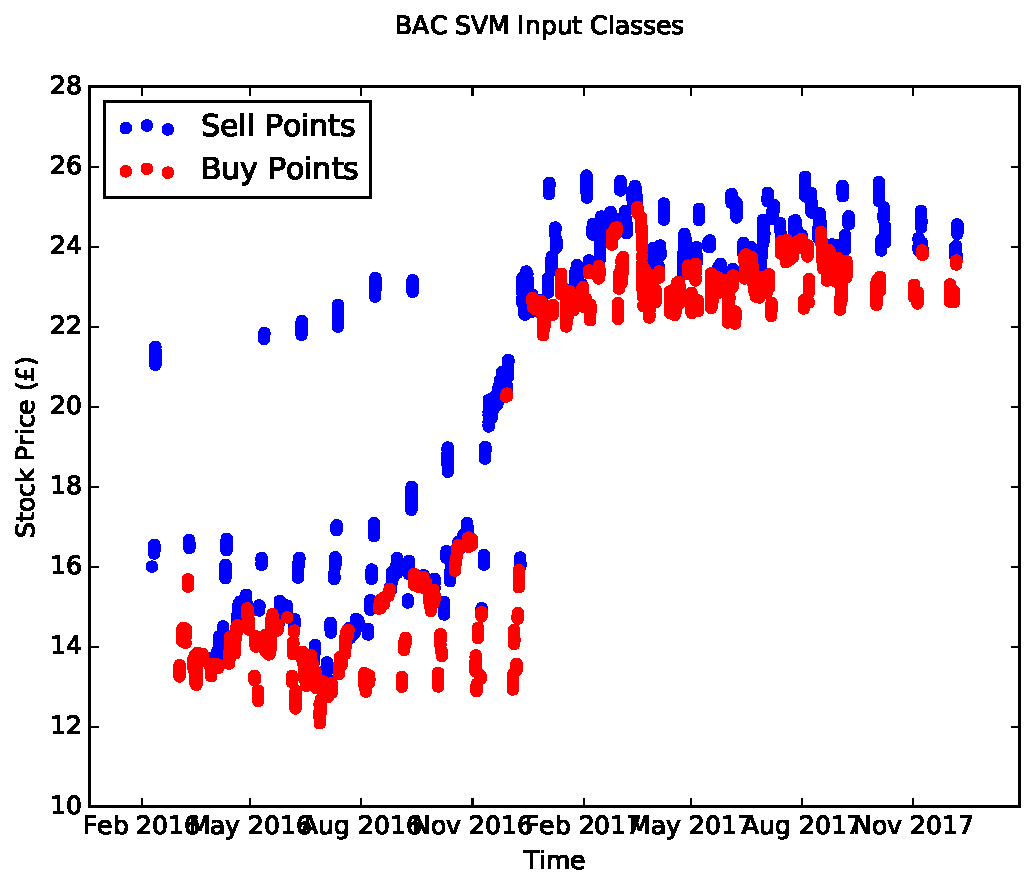
\includegraphics[width=0.5\textwidth, angle=0]{Poster/SVMBuyPoints.pdf}
\caption{A graph showing the resulting data of the `spikes' technique used to create the input data for both SVMs.}
\label{fig:SVMBuyPoints}
\end{figure}

\subsubsection{Query}

The query function within the e1071 library is very simple, given an SVM that has learnt its separator a function call will return the group that the given point belongs to.

This system is managed within the `shouldBuy' and `shouldSell' functions that were discussed within the statistical methods section. These have been modified so as to retrain and query the `shouldBuySVM' and the `shouldSellSVM' each time that they are called. Firstly one of these functions will be called within the simulation, for simplicity, `shouldBuy' will be used as an example. `shouldBuy' is called, within this function is the call to create and train the SVM associated with this function, namely `shouldBuySVM', trained on the dataframe that is shown in table \ref{fig: Table SVM Buy Data}. The data within this dataframe has been continuously updated throughout the simulation so as to avoid bulk computation when the SVM is used. This is done by continual calls to the `getPeaks' function on regular intervals. Once the SVM has been trained, it is queried with the latest price for the given stock. This will return a class and then a decision will be made based on the class that has been returned.

\iffalse
#################################################################################
\fi

\section{Results and Evaluation}

\iffalse
this section presents the results of the solutions.  It should include information on experimental settings.  The results should demonstrate the claimed benefits/disadvantages of the proposed solutions.
This section should be between 2 to 3 pages in length.

- Testing Criteria for each of the stat methods\\
- decision criteria for each of the peak trough methods\\
- input variables for the SVM - kernal etc \\
- conjunction test criteria for each of the good stat methods\\
- best stat method result possible\\
- best ml method result possible

This section should between 1 to 2 pages in length.
\fi

The statistical methods throughout this paper have been tested in slightly different ways, as explained within the testing section. This will be outlined for each of the methods. The machine learning methods will also be outlined but individually.\\

\subsection{Technical Overlays}

\textbf{Bollinger Bands} - Buy criteria will be based on percentage values in conjunction with the spread of the upper and lower band, giving an indication of volatility. The sell criteria is purely based on the relationship between the current price and middle band. Single variable of X was tested at X = 20, 15, and 35, with 20 being the default.

\textbf{Chandelier Exit} - The buy criteria is based on the relationship between the current moving average and the stock price at any given moment. The sell criteria are purely based on the conjunction between the long and short values of this overlay. Single variable of X was tested at X = 22, 17, and 27, with 22 being the default.

\textbf{Ichimoku Cloud} - The buy and sell criteria are based on the relationship between the A and B leading span with the other values providing momentum information. This has five variables and was not tested at any other values besides default.

\textbf{KAMA} - Allowing for clear identification of turning points, the buy and sell criteria are based on the difference between the KAMA value and the stock price. This has three variables and was not tested at any other values besides default.

\textbf{Keltner Channels} - Uses the same criteria as Bollinger Bands just with slightly different behaviour due to the differences between them. Takes two variables with default X = 20 and Y = 10, was tested at (15, 10), (25, 10), (20, 5), and (20, 15).

\textbf{Moving Averages} - Both Exponential and Simple moving averages were tested with basic comparison filters to give buy and sell criteria. Takes a single input and has no default, was tested at 5, 10, 15, 20, 25, and 30.

\textbf{Moving Averages Envelopes} - The buy criteria are based on the relationship between stock price and the lower envelope with the sell criteria being based on the relationship between the stock price and upper envelope. Takes two variables with default X = 20 and Y = 0.025. Tested at (15, 0.025) and (25, 0.025).

\textbf{Parabolic SAR} - Tracking of rising and falling SAR values gives an inference as to the correct time to buy and sell and these have been used as the criteria. This has no variables to be tested.

\textbf{Pivot Points} - The criteria for all three types of pivot point are similar with the only caveat being the number of support and resistance values that are taken into consideration as the buy and sell criteria change along with the value of the pivot point. These were only tested at default configurations.

\textbf{Price Channels} - Buying criteria is based on a moving average value in conjunction with a downward trend. Selling criteria is based purely on an inverting upward trend. These channels take a single variable with default value of 20, was then tested at 15 and 25 as well.

\subsection{Technical Indicators}

\textbf{Aroon} - Buy and sell criteria both based on the relationship between a moving average and the current stock price in conjunction with the trend information provided by the relationship between the up and down values. Single input value tested at 25 (default), 20, and 30.

\textbf{Aroon Oscillator} - Very similar to the Aroon test criteria but instead of using the relationship between up and down only the oscillator value is used. Single input tested at 25 (default), 20, and 30.

\textbf{Average True Range} - Using a moving average with bounded buy and sell criteria, ATR is used to indicate volatility of the price at a given point and this will impact the bounds used. This has no variables that needed to be tested. 

\textbf{BandWidth} - Buy and sell are both based on percentage criteria of the bandwidth value as it is an inference of Bollinger Bands. Using Bollinger Bands as a base, this has a single input and was tested at 20 (default), 15, and 25.

\textbf{\%B Indicator} - The same as BandWidth as they are both Bollinger Band derivatives. Both derivatives were tested at the same values as well.

\textbf{Commodity Channel Index} - Percentage criteria for buy and sell using the final CGI value. Taking a single input variable that was tested at 20 (default), 15, and 25.

\textbf{Coppock Curve} - The buy criteria is based on a moving average and the stock price; the sell criteria was based on the sign of the indicator. This takes three variables and was only tested at the default values.

\textbf{DecisionPoint Price Momentum Oscillator} - Using the value of the indicator in conjunction with a moving averages relationship with the stock price; buy is based on the moving averages relationship and is not cut short by using the momentum indicator. The same is done in the inverse for sell. This was only tested at the default values.

\textbf{Detrended Price Oscillator} - This was tested and found to have limited use as a single indicator. Takes a single input and was tested at 15, 20, 25, and 30.

\textbf{Mass Index} - The buy and sell criteria are based on the calculation of the current trend and then use the indicator to show a trend reversal before the trend changes. This was tested at default values.

\textbf{Moving Average Convergence/Divergence Oscillator} - Used within the buy and sell criteria in the same way as all other momentum oscillators; in conjunction with a moving average and bounds. This was tested at default values.

\textbf{MACD Histogram} - Used identically to MACD, with the limited availability of inter-value relationship information. This was tested at default values. 

\textbf{Percentage Price Oscillator} - Percentage bound for buy and sell criteria based on previous values of the PPO. This was tested at default values.

\textbf{Pring's Know Sure Thing} - Another momentum oscillator tested in conjunction with a moving average. This was tested at default values.

\textbf{Pring's Special K} - Using a percentage bound based around past values to give an indication of movement prediction. This was tested at default. 

\textbf{Rate of Change and Momentum} - Used in conjunction with a moving average, this most basic momentum oscillator is the foundation for most of the more advance versions and so is tested in the same way. This takes a single input with no default and was tested at 5, 10, 20, 30, 50, and 100.

\textbf{Relative Strength Index} - Using previous values of RSI, bounds are calculated at the upper and lower range of the value 0 to 100 to give an indicator of the optimal times to buy and sell. The bounds have an initial value and are changed based on the data. This takes a single input with 10, 20, and 30 being tested.

\textbf{StockCharts Technical Rank} - Using the final value of SCTR, as well as the relationship between individual components, a confidence is calculated with respect to the changing of the price, as well as the direction of the change. This was only tested at default values.

\textbf{Slope} - Using the current slope value over the last set number of data points an inference can be made as to the future direction of the stock price. This projection is then used to indicate buying and selling patterns. Taking a single input, this was tested at 10, 20, and 30.

\textbf{Stochastic Oscillator} - Using the momentum value in conjunction with a moving average, confidence in the projection of price is known and thus buy and sell behaviour is simple. This takes two input values, with defaults (14, 3), this was tested along with (12, 3), (16, 3) and (14,2), (14, 4).

\textbf{StochRSI} - Using the previous values of the indicator upper and lower bounds are calculated to allow for the inference of buying and selling behaviour. This takes a single input with a default value of 14, this was tested, as was 10, 12, 16, and 18.

\textbf{TRIX} - Using percentage bounds, the current TRIX value is compared to a set of previous TRIX values and decisions on buying and selling are made based on this relationship. This takes a single input and was tested at 10, 20, and 30. 

\textbf{True Strength Index} - Using percentage bounds based on previous TSI values, buying and selling behaviour is inferred. With two input values, the default (25, 13) was tested. As was (20, 13) and (30, 13).

\textbf{Ulcer Index} - The volatility shown using this indicator is used with regard to bounds initially set over a moving average and altered to reflect the volatility of the market. A single input, with default value 14, was tested along with 10 and 18.

\textbf{Ultimate Oscillator} - The smoothed momentum that this indicator shows is used in addition to a moving average to allow for inference within a trend to show turning points within the data and reduce the possibility of leaving a trend early. This takes three input variables that were tested at (7, 14, 28), (6, 12, 24), and (8, 16, 32), with the first being the default values.

\textbf{Vortex Indicator} - The relationship between the two oscillators calculated is used as trend and momentum information and all behaviours are inferred from these values and their relationship. With single input default value of 14, 10 and 18 were tested as well.

\textbf{Williams \%R} - Used in an identical way to the Stochastic Oscillator, as this is an inference of that. Taking a single input value, along with the default 14, 10, and 18 were also tested.

\subsection{Support Vector Machines}

The first part of the testing of the support vector machine, or SVM, was to perform a search over variable space to find the best variables to use for testing. The variables that need to be tested consist of the data manipulation to start with, then the kernel that was to be used, as well as degree, C, and gamma, which are inputs to the function. These are all used within each of the SVMs, each of which are since class classifiers. 

Data manipulation was split into differentiation, rolling average, spikes, and median (as discussed in section C.1). The kernel choice, also discussed in section C.1, is between a linear kernel, polynomial kernel, sigmoid function, and a radial basis function. These are all available through the e1071 library \cite{Meyer2017}. The degree, C value, and gamma are all searched via the library's built-in grid search function. 

\subsection{Results}

This section shows the best results that could be achieved within three sections of the paper. The first section is a purely statistical method used alone. The second is a conjunction of two or more statistical methods. The third is any formulation of support vector machine. These are shown in tables \ref{fig: Table Individual Results}, \ref{fig: Table Conjunction Results}, and \ref{fig: Table SVM Results}, respectively.

The aim of the project was to achieve a higher percentage in a given time frame that would be available from a high street bank. The values of which were set at 0.5\% at the lowest \cite{BankofEngland2014} and 1.85\% at the highest \cite{Murray2018}. As is clearly shown in Table  \ref{fig: Table Individual Results} the use of any of the top ten statistical measures is enough to achieve this goal using even the highest fixed percentage individual savings accounts over the same time frame. The individual method results are then surpassed by the conjunction results show in Table \ref{fig: Table Conjunction Results}, which are then again surpassed by the results of the SVM seen in Table \ref{fig: Table SVM Results}.

The most successful results actions are shown in figure \ref{fig:SVMResults}. This shows the points at which the most successful SVM bought and sold this specific stock. This gives an indication as to the success of this algorithm. The reason for no actions being made in the first six months is due to this being designated as a learning period and is not within the allotted trading time frame.

\begin{figure}
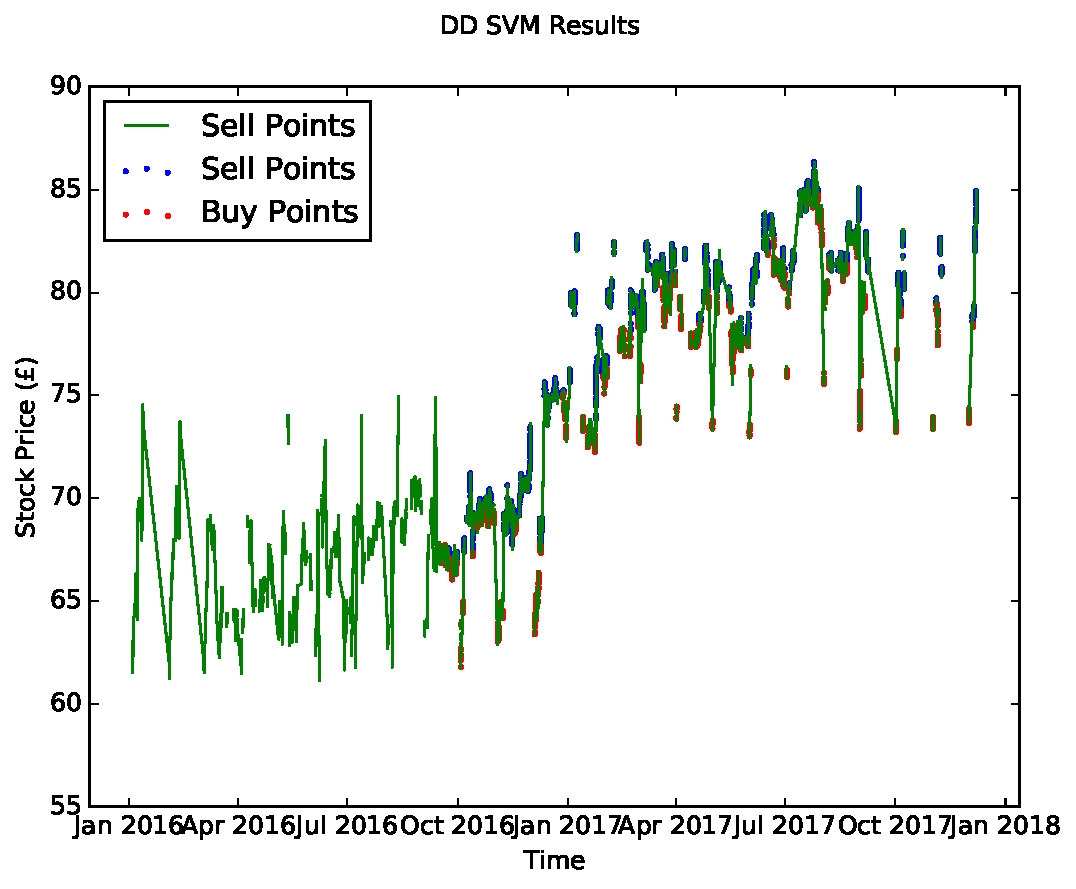
\includegraphics[width=0.5\textwidth, angle=0]{SVMResults.pdf}
\caption{A graph showing the buying and selling points of both SVMs trained on the stock DD, as well as the stock price of DD.}
\label{fig:SVMResults}
\end{figure}

\begin{table*}
\centering
\begin{tabu}{ |p{4cm}|p{4cm}|p{4cm}|}\hline\hline
Method & Parameters & Result \\ \hline
Parabolic SAR & Default & 8.94\% \\ \hline
KAMA & Default & 8.29\% \\ \hline
Ichimoku Cloud & Default & 8.02\% \\ \hline
MACD & Default & 7.12\% \\ \hline
Mass Index & Default & 6.78\% \\ \hline
Bollinger Bands & 25 & 5.83\% \\ \hline
StockCharts Technical Rank & Default & 5.41\% \\ \hline
DecisionPoint Price Momentum Oscillator & Default & 5.16\% \\ \hline
Stochastic Oscillator & 14, 4 & 4.92\% \\ \hline
Pivot Points & Default & 2.19\% \\ \hline
\end{tabu}
\vspace{2 mm}
\caption{Top 10 Individual Results}
\label{fig: Table Individual Results}
\end{table*}

\begin{table*}
\centering
\begin{tabu}{ |p{4cm}|p{4cm}|p{4cm}|}\hline\hline
Methods & Parameters & Result \\ \hline
MACD + KAMA & Default, Default & 11.39\% \\ \hline
Bollinger Bands + DecisionPoint Price Momentum Oscillator & 25, Default & 11.23\% \\ \hline
MACD + Parabolic SAR & Default, Default & 10.86\% \\ \hline
MACD + Mass Index & Default, Default & 10.84\% \\ \hline
Stochastic Oscillator + KAMA & 14, 4, Default & 10.83\% \\ \hline
MACD + Pivot Points & Default, Default & 10.44\% \\ \hline
Stochastic Oscillator + Parabolic SAR & 14, 4, Default & 8.18\% \\ \hline
Bollinger Bands + KAMA & 25, Default & 6.96\% \\ \hline
StockCharts Technical Rank + Parabolic SAR & Default, Default & 6.19\% \\ \hline
Bollinger Bands + Pivot Points & 25, Default &  6.02\%\\ \hline
\end{tabu}
\vspace{2 mm}
\caption{Top 10 Conjunction Results}
\label{fig: Table Conjunction Results}
\end{table*}

\begin{table*}
\centering
\begin{tabu}{ |p{4cm}|p{4cm}|p{4cm}|}\hline\hline
Method & Parameters & Result \\ \hline
SVM & Differentiation + Sigmoid Function & 18.41\% \\ \hline
SVM & Median + Sigmoid Function & 17.98\% \\ \hline
SVM & Rolling Average + Sigmoid Function & 16.17\% \\ \hline
\end{tabu}
\vspace{2 mm}
\caption{Top Three Support Vector Machine Results}
\label{fig: Table SVM Results}
\end{table*}

\iffalse
#################################################################################
\fi

\section{Conclusions}

\iffalse
This section summarises the main points of this paper.  Do not replicate the abstract as the conclusion.  A conclusion might elaborate on the importance of the work or suggest applications and extensions.  This section should be no more than 1 page in length.

- extend the number of stat methods used \\
- test using more data, multiple sources, more complete, more fine grain \\
- test more ML methods - NN or K-Means or Genetic algorithm for each stock\\
- use live data? \\
- stop and put? \\
\fi

This section outlines the trends seen within the results that this paper has found and will also discuss the possible routes that could be taken if this project were to be extended.

\subsection{Trends}

As the results in Table \ref{fig: Table Individual Results} so clearly show it is very possible to outstrip the target set by a typical high street bank, using only statistical methodology. The table also shows a clear bias towards functions that base their methodology around the identification of the end of trends and the resultant information provided. This is a general trend however as there are several that are not based around this idea. Instead they are complete packages that calculate momentum and trend information and use it within either long-reaching or complex systems. 
Another trend is seen in Table \ref{fig: Table Conjunction Results}, the conjunction of a method based around the identification of trends and another method based around more complex moving averages give very promising results. 
The final results in Table \ref{fig: Table SVM Results} gives a clear indication as to the best direction for future research. The benefits of machine learning within this context cannot be overstated. The results of the best of the SVM tests clearly show that statistical methods have a place within this field, it is just relegated to data manipulation to help improve the input for machine learning techniques.\\

\subsection{Extension}

An extension to this project that would be a boon to the testing would be a finer granularity of data. The data used in this paper was limited by the financial aspect of data acquisition; the paper and its findings were not hindered in this but it was a known limiting factor. Another data extension to be  considered is the use of live data. This data would be taken periodically from a stock exchange to provide a more realistic approach to live trading. We maintain the statement that statistical methods are useful and will be needed no matter how advanced the project's machine learning techniques become. The number of data manipulation and extraction techniques that would be tested would increase: this is an open-ended task as no data would be perfect. The final extension to the would be testing a wider range of machine learning techniques. The use of deep learning within contemporary computer science is significant and this would be an obvious next step for this area.

\iffalse
#################################################################################
\fi

\bibliography{references}

\nocite{*}

\iffalse
#################################################################################
\fi

\iffalse
\section*{------------------------------------------------------------}

\subsection{Main Text}

The font used for the main text should be Times New Roman (Times) and the font size should be 12.  The first line of all paragraphs should be indented by 0.25in, except for the first paragraph of each section, subsection, subsubsection etc. (the paragraph immediately after the header) where no indentation is needed.

\subsection{Figures and Tables}
In general, figures and tables should not appear before they are cited.  Place figure captions below the figures; place table titles above the tables.  If your figure has two parts, for example, include the labels ``(a)'' and ``(b)'' as part of the artwork.  Please verify that figures and tables you mention in the text actually exist.  make sure that all tables and figures are numbered as shown in Table \ref{units} and Figure 1.
%sort out your own preferred means of inserting figures

\begin{table}[htb]
\centering
\caption{UNITS FOR MAGNETIC PROPERTIES}
\vspace*{6pt}
\label{units}
\begin{tabular}{ccc}\hline\hline
Symbol & Quantity & Conversion from Gaussian \\ \hline
\end{tabular}
\end{table}

\subsection{References}

The list of cited references should appear at the end of the report, ordered alphabetically by the surnames of the first authors.  References cited in the main text should use Harvard (author, date) format.  When citing a section in a book, please give the relevant page numbers, as in \cite[p293]{budgen}.  When citing, where there are either one or two authors, use the names, but if there are more than two, give the first one and use ``et al.'' as in  , except where this would be ambiguous, in which case use all author names.

You need to give all authors' names in each reference.  Do not use ``et al.'' unless there are more than five authors.  Papers that have not been published should be cited as ``unpublished'' \cite{euther}.  Papers that have been submitted or accepted for publication should be cited as ``submitted for publication'' as in \cite{futher} .  You can also cite using just the year when the author's name appears in the text, as in ``but according to Futher \citeyear{futher}, we \dots''.  Where an authors has more than one publication in a year, add `a', `b' etc. after the year.

\iffalse
#################################################################################
\fi

\begin{table}[htb]
\centering
\caption{SUMMARY OF PAGE LENGTHS FOR SECTIONS}
\vspace*{6pt}
\label{summary}
\begin{tabular}{|ll|c|} \hline
& \multicolumn{1}{c|}{\bf Section} & {\bf Number of Pages} \\ \hline
I. & Introduction & 2--3 \\ \hline
II. & Related Work & 2--3 \\ \hline
III. & Solution & 4--7 \\ \hline
IV. & Results & 2--3 \\ \hline
V. & Evaluation & 1-2 \\ \hline
VI. & Conclusions & 1 \\ \hline
\end{tabular}
\end{table}

\iffalse
#################################################################################
\fi

\section*{Notes for the final paper}

\subsection*{Data}
- taken from a website
- between dates
- in format
- using R and shell scripts managed
- put into a single file
- read in
- initially had an issue with data, not enough
- was rectified and the same steps were followed to put it in the same format
- dumbing of the data was done ? might not mention this but we only take the open price of each minute, thus reducing the dataload, this would not be done in a full scale system as we would have all the metrics and data from the past and all maths that would be used has already been calculated.

\subsection*{Notes}
- ghomas has suggested that we run the code on the GPU as we are running a rolling average
- It could be run on hamilton
- This will take some research but we will continue in the research department first
- Then we will do this parallelism
- then we will implement some of the researched techniques

- the functions we need to implement are:
- when to buy
- when to sell
- how much to buy

- a buy and hold strategy could be implemented first, this would be a buy early in the year and hold until the end, any short term fluctuations would not have any effect but the exact time to buy and sell could be tricky, this in an initial buy at a low price and a late sell at a high price, any fluctuations in the middle are not important only the difference in almost the whole market as this is a conservative approach to trading and will spread the bet.

- genetic trading algorithm, this is more of a technique to make a strategy rather than a strategy itself, the idea is to 'learn' how to trade, using a fitness function and other such techniques on a strategy that is already in place in order to fine tune it. This may be hard to implement but could have some merit.

- there is the possibility of making some machine learning algorithms that will do the same thing, this will have to be researched in R as this is new to me. The techniques are not, but the language in conjunction is.

- some hands on trading strategies could be considered, just with the algorithm being the active party not the person. These include position trading, swing trading, scalping, and day trading. These can be considered.

- alpha is something that may be useful, it is a metric used to measure risk. Alpha is one of five technical risk ratios; the others are beta, standard deviation, R-squared, and the Sharpe ratio. All these will be looked into, to see if any benefit can be drawn from them. They may be useful in later calculations.
\fi

\end{document}